
\chapter{Linear Algebra Arithmetic}

This chapter covers the following ideas. 


\begin{enumerate}

\item Be able to use and understand matrix and vector notation, addition, scalar multiplication, the dot product, matrix multiplication, and matrix transposition. 
\item Use Gaussian elimination to solve systems of linear equations and write the solution in parametric and vector form. Define and use the words homogeneous, nonhomogeneous, row echelon form, and reduced row echelon form. 
\item Find the rank of a matrix. Determine if a collection of vectors is linearly independent. If linearly dependent, be able to write vectors as linear combinations of the preceding vectors.
\item For square matrices, compute determinants, inverses, eigenvalues, and eigenvectors. 
\item Illustrate with examples how a nonzero determinant is equivalent to having independent columns, an inverse, and nonzero eigenvalues. Similarly, a zero determinant is equivalent to having dependent columns, no inverse, and a zero eigenvalue. 

\end{enumerate}

%%% Local Variables: 
%%% mode: latex
%%% TeX-master: "../linear-algebra"
%%% End: 


The next unit will focus on applications of these ideas. The main goal of this unit is to familiarize yourself with the arithmetic involved in linear algebra.

\section{Basic Notation}
Most of linear algebra centers around understanding matrices and vectors. The first chapter of this text contains a brief introduction to the arithmetic involved with matrices and vectors.  The second chapter will show you many real-world applications of the ideas we are learning.  For now, work on becoming familiar with the arithmetic of linear algebra so that we can easily discuss the ideas behind linear algebra throughout the course.


\subsection{Matrices}
\marginpar{
Matrix size is

row by column.} 
A \define{matrix} of size ``{$m$} by {$n$}'' ($m\times n$) is a table
with {$m$} rows and {$n$} columns.  We normally give matrices names
using capital letters, and use the notation 
$$A = 
\begin{bmatrix}
a_{11}&\cdots&a_{1n}\\ 
a_{21}&\cdots&a_{2n}\\ 
\vdots&\ddots&\vdots\\ 
a_{m1}&\cdots&a_{mn} 
\end{bmatrix} 
= [a_{jk}],$$
where $a_{jk}$ is the entry in the $j$th row and $k$th column. 


We say two matrices {$A$} and {$B$} are equal if corresponding entries
are equal (i.e., {$a_{jk}=b_{jk}$} for all $j$ and $k$). We add and
subtract matrices of the same size entry-wise.  A \define{scalar} is a
single number or variable.  We multiply a scalar and a matrix $cA$ by multiplying every entry in the matrix by the scalar {$c$}. If the number of rows and columns are equal, then we say the matrix is square.  The main \define{diagonal} of a square ({$n \times n$}) matrix consists of the entries {$a_{11},a_{22},\ldots,a_{nn}$}, and the \define{trace} is the sum of the entries on the main diagonal ($\sum a_{jj}$).
\begin{example}
If $A=\begin{bmatrix}
1&3\\
0&2
\end{bmatrix}
$ and 
$B=
\begin{bmatrix}
3&-1\\
0&4
\end{bmatrix}
$, then $$A-2B
=\begin{bmatrix}
1-2\cdot3&3-2\cdot(-1)\\
0-2\cdot 0& 2-2\cdot 4
\end{bmatrix}
=\begin{bmatrix}
-5&5\\
0&-6
\end{bmatrix}.$$ The main diagonal of $B$ consists of the entries $b_{11} = 3$ and $b_{22}=4$, which means the trace of $B$ is $3+4=7$ (the sum of the entries on the main diagonal).
\end{example}

\begin{example}
Let $A=\begin{bmatrix}
\fbox{3}&2&1\\
-2&\fbox{-1}&5\\
4&7&\fbox{9}
\end{bmatrix}$.  The diagonal of a square matrix is the list of entries from upper left diagonally to lower right: $3,-1,9$ (we've emphasized this by drawing boxes around the diagonal entries).  The trace is 11.
\end{example}

The \definemargin{transpose} of a matrix {$A=[a_{jk}]$} is a new matrix {$A^T=[a_{kj}]$} formed by interchanging the rows and columns (the first row of $A$ is the first column of $B$; first column of $A$ is the first row of $B$, etc.)
%Notice that {$(AB)^T = B^TA^T$}, which follows immediately if you realize that the {$j$}th row of {$A$} and {$k$}th column of {$B$} become the {$k$}th row of {$B^T$} and {$j$}th column of {$A^T$}. 
\begin{example} \label{ex transpose}
The transpose of $A$ is illustrated below.
$$\begin{array}{ccc}
A =\begin{bmatrix} 0&1&-1\\1&0&2
\end{bmatrix}, &
A^T = \begin{bmatrix} 0&1\\1&0
\\-1&2\end{bmatrix} 
\end{array}.$$
\end{example}
%The following names are given to special kinds of square matrices.
%\begin{enumerate}
%	\item Identity matrix: 1's on the diagonal and 0's everywhere else. This matrix plays the role of the number one in matrix multiplication, as {$IA=AI=A$}.
%\item Symmetric if {$A^T=A$}.
%\item Skew-symmetric if {$A^T=-A$} (which means the diagonal entries are all zero).
%\item Upper triangular if nonzero entries occur on or above the the main diagonal.
%\item Lower triangular if nonzero entries occur on or below the the main diagonal.
%
%\end{enumerate}
%$$\begin{array}{ccccc}
%\begin{bmatrix} 1&0&0\\0&1&0
%\\0&0&1\end{bmatrix} 
%&\begin{bmatrix} 1&3&2\\3&4&0
%\\2&0&-1\end{bmatrix} 
%&\begin{bmatrix} 0&-3&1\\3&0&2
%\\-1&-2&0\end{bmatrix} 
%& \begin{bmatrix} 1&3&2\\0&4&0
%\\0&0&-1\end{bmatrix} 
%& \begin{bmatrix} 1&0&0\\3&4&0
%\\2&0&-1\end{bmatrix} \\
%\text{identity}
%&\text{symmetric}
%&\text{skew-symmetric}
%&\text{upper-triangular}
%&\text{lower-triangular}
%\end{array}$$
%
%


\subsection{Vectors}
Vectors represent a magnitude in a given direction. We can use vectors to model forces, acceleration, velocity, probabilities, electronic data, and more. We can use matrices to represent vectors. A row vector is a {$1\times n$} matrix. A column vector is an {$m \times 1$} matrix.   Textbooks often write vectors using bold face font. By hand (and in this book), we write an arrow above them. The notation ${\bf v} = \vec v = \left<v_1,v_2,v_3\right>$ can represent either a row or column vector. Many different ways to represent vectors are used in different books.  For example, you may see the vector $\left<-2,3\right>$ written in any of the following ways.
$$\left<-2,3\right>
= -2{\bf i}+3{\bf j} 
= (-2,3) 
= \begin{bmatrix}-2&3\end{bmatrix} 
= \begin{bmatrix}-2\\3\end{bmatrix}
= \begin{pmatrix}-2&3\end{pmatrix} 
= \begin{pmatrix}-2\\3\end{pmatrix}
$$ 
In this chapter, we will switch freely between these notations so that you get used to reading different notations.  In practice, it is a good idea to not switch notations as often to avoid confusion.  Also, notice that the notation $(-2,3)$ (with parentheses) has other meanings as well (like a point in the plane, or an open interval).  Please make sure that when you use the notation $(-2,3)$ to represent a vector, it is clear from the context that you working with a vector. 

{\marginpar{{
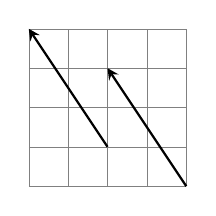
\begin{tikzpicture}[scale=.5]
\draw[help lines,step=1cm] (0,0) grid (4,4);
\draw[->,>=stealth,thick] (2,1) -- (0,4);
\draw[->,>=stealth,thick] [xshift=2cm, yshift=-1cm](2,1) -- (0,4);
\end{tikzpicture}

Both vectors 
represent $\left<-2,3\right>$, regardless of where they start.
}}}
To draw a vector, pick a starting point (the tail).  Then draw a line that moves $v_1$ units horizontally and $v_2$ units vertically, and put an arrow at the ending point (the head).  Many times we will put the tail of the vector at the origin ($(0,0)$ for 2-d vectors).


The entry-wise methods of adding, subtracting, and multiplying by a scalar that we learned for matrices apply to vectors as well (this is consistent, since a vector can be thought of as a row or column matrix). For example, $$\left<1,3\right>-2\left<-1,2\right>+\left<4,0\right> = \left<1-2(-1)+4,3-2(2)+0\right> = \left<7,-1\right>.$$ 
Sometimes it is easier to see the arithmetic if we write the vectors as single-column matrices:
$$
\begin{bmatrix}1\\3\end{bmatrix}
-2\begin{bmatrix}-1\\ 2\end{bmatrix}
+ \begin{bmatrix}4\\0\end{bmatrix}
= \begin{bmatrix}1-2(-1)+4\\3-2(2)+0\end{bmatrix}
= \begin{bmatrix}7\\-1\end{bmatrix}.
$$

\marginpar{{%\normalsize
\begin{center}
Vector Addition

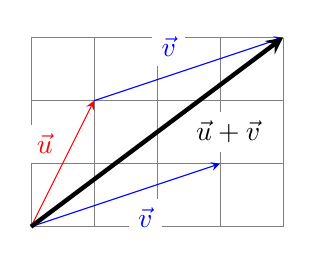
\begin{tikzpicture}[scale=.8]
\draw[help lines,step=1cm] (0,0) grid (4,3);
\draw[->,>=stealth,red] (0,0) -- node[above left ,fill=white] {$\vec u$}(1,2);
\draw[->,>=stealth,blue] (0,0) -- node[below right=1pt,fill=white] {$\vec v$} (3,1);
\draw[->,>=stealth,blue] [shift={(1,2)}](0,0) -- node[above left=1pt,fill=white]{$\vec v$} (3,1);
\draw[->,>=stealth,ultra thick] (0,0) -- node[right=10pt,fill=white] {$\vec u+\vec v$}(4,3);
\end{tikzpicture}
\end{center}

%\marginpar{{%\normalsize
\begin{center}
Scalar Multiplication

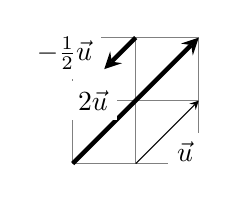
\begin{tikzpicture}[scale=.8]
\draw[help lines,step=1cm] (-1,0) grid (1,2);
\draw[->,>=stealth] (0,0) -- node[below right ,fill=white] {$\vec u$}(1,1);
\draw[->,>=stealth,ultra thick] [xshift=-1cm,scale=2](0,0) -- node[left=6pt ,fill=white] {$2\vec u$}(1,1);
\draw[->,>=stealth,ultra thick] [yshift=2cm,scale=-.5](0,0) -- node[left=6pt ,fill=white] {$-\frac12\vec u$}(1,1);
\end{tikzpicture}
\end{center}
%}}

%\marginpar{{%\normalsize
\begin{center}
Vector Subtraction

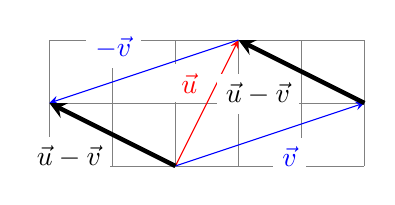
\begin{tikzpicture}[scale=.8]
\draw[help lines,step=1cm] (-2,0) grid (3,2);
\draw[->,>=stealth,red] (0,0) -- node[above left ,fill=white] {$\vec u$}(1,2);
\draw[->,>=stealth,blue] (0,0) -- node[below right=1pt,fill=white] {$\vec v$} (3,1);
\draw[<-,>=stealth,blue] [shift={(-2,1)}](0,0) -- node[above left=1pt,fill=white]{$-\vec v$} (3,1);
\draw[->,>=stealth,ultra thick] (0,0) -- node[below left=0pt,fill=white] {$\vec u-\vec v$}(-2,1);
\draw[->,>=stealth,ultra thick] [shift={(3,1)}](0,0) -- node[below left=0pt,fill=white] {$\vec u-\vec v$}(-2,1);
\end{tikzpicture}
\end{center}
%}}

}}Vector addition is performed geometrically by placing the tail of the second vector at the head of the first. 
The resultant vector is the vector which starts at the tail of the first and ends at the head of the second. This is called the parallelogram law of addition. The sum $\vec u + \vec v=\left<1,2\right> + \left<3,1\right> = \left<4,3\right>$ is illustrated in the margin.

Scalar multiplication $c\vec u$ ($c$ is a scalar and $\vec u$ is a vector) is equivalent to stretching (scaling) a vector by the scalar without rotating the vector. The product $2\vec u$ doubles the length of the vector. If the scalar is negative, then the vector reverses to point in the opposite direction.  The product $-\frac{1}{2}\vec u$ is a vector half as long as $\vec u$ and points in the opposite direction (as illustrated in the margin).

To subtract to vectors $\vec u-\vec v$, we use scalar multiplication and vector addition.  We write $\vec u-\vec v = \vec u +(-\vec v)$, which means we reverse $\vec v$ and then add it to $\vec u$.  You can visualize this using the parallelogram law of addition.  You can also visualize the difference $\vec u-\vec v$ as the vector connecting the heads of the two vectors when their tails are both placed on the same spot, with the direction pointing towards the head of $\vec u$.  When you see a vector difference $\vec u-\vec v$, you might imagine an arrowhead on the subtraction sign like this: $\vec u \leftarrow \vec v$, or think ``head  minus tail'' to remind you which way the difference vector points. The difference $\vec u - \vec v=\left<1,2\right> - \left<3,1\right> = \left<-2,1\right>$ is illustrated in two vectors in the margin.

\subsection{Magnitude and the Dot Product}
The length of a vector is found using the Pythagorean theorem: $c^2=a^2+b^2$.  The \define[vector!magnitude]{magnitude} (or length) of the vector $\left<2,3\right>$ is simply the length of the hypotenuse of a right triangle with short side lengths 2 and 3, hence $\norm{\left<2,3\right>}=\sqrt{2^2+3^2}=\sqrt{13}$. We denote magnitude with absolute value symbols, and compute for $\vec u = \left<u_1,u_2\right>$ the magnitude as $\norm{\vec u} = \sqrt{u_1^2+u_2^2}$.  In higher dimensions we extend this as $$\ds \norm{\vec u} = \sqrt{u_1^2+u_2^2+u_3^2+\cdots u_n^2} = \sqrt{\sum_{i=1}^n u_i^2}.$$ 

A unit vector is a vector with length 1. 
\marginpar{A unit vector $\bf \hat u$ has length $\norm{\bf \hat u}=1$} In many books, unit vectors are written with a hat above them, as $\bf{\hat u}$.
Any vector that is not a unit vector can be rewritten as a scalar times a unit vector by dividing the vector by its magnitude. This allows us to write any vector as a magnitude times a direction (where the direction is given by a unit vector).
 
\begin{example}
The length of $\vec u=\left<2,1,-3\right>$ is $\sqrt{2^2+1^2+(-3)^2} = \sqrt{4+1+9}=\sqrt{14}$.  
A unit vector in the direction of $\vec u$ is 
$\ds\frac{1}{\sqrt{14}}\left<2,1,-3\right> = \left<\frac{2}{\sqrt{14}},\frac{1}{\sqrt{14}},\frac{-3}{\sqrt{14}}\right>$. 
We can rewrite $\vec u$ as a magnitude times a direction by writing 
\marginpar{Every vector can be rewritten as a magnitude times direction (unit vector).}
$$\vec u = \norm{\vec u} \frac{\vec u}{\norm{\vec u}} = \sqrt{14} \left<\frac{2}{\sqrt{14}},\frac{1}{\sqrt{14}},\frac{-3}{\sqrt{14}}\right>.$$ 
\end{example}


The \define[vector!dot product]{dot product} of two vectors $\vec u = \left<u_1,u_2,\ldots,u_n\right>$ and $\vec v =\left<v_1,v_2,\ldots,v_n\right>$ is the scalar given by multiplying corresponding components and adding the products together (i.e., $\vec u\cdot \vec v = u_1v_1+u_2v_2+\cdots+u_nv_n = \sum u_iv_i$).
\begin{example} \label{ex dot product}
The dot product of $\begin{bmatrix}1&3&-2\end{bmatrix}$ and $\begin{bmatrix}2&-1&4\end{bmatrix}$ is
 $$\begin{bmatrix}1&3&-2\end{bmatrix}\cdot \begin{bmatrix}2&-1&4\end{bmatrix} = (1)(2)+(3)(-1)+(-2)(4)=-9.$$ 
\end{example}

We use the dot product to find lengths and angles in all dimensions. We will also use it multiply matrices.  The rest of this section explains how to use the dot product to find lengths and angles.  We will revisit the dot product more in later chapters.
Notice that if $\vec u = \left<u_1,u_2,\ldots,u_n\right>$, then we can find the length of a vector using the dot product since
\marginpar{The dot product finds length: $$\vec u\cdot \vec u = \norm{\vec u}^2$$}
$$\vec u\cdot \vec u = u_1^2+u_2^2+u_3^2+\cdots u_n^2 = \sum_{i=1}^n u_i^2 = \norm{\vec u}^2.$$
If $\theta$ is the angle between two vectors $\vec u$ and $\vec v$, then we can find the angle between these two vectors using the formula \marginpar{The dot product finds angles: $$\vec u \cdot \vec v = \norm{\vec u}\norm{\vec v}\cos \theta$$}
$$\vec u \cdot \vec v = \norm{\vec u}\norm{\vec v}\cos \theta.$$
This follows from the law of cosines $c^2 = a^2 + b^2 -2ab \cos \theta$, where $a=\norm{\vec u}$, $b=\norm{\vec v}$, and $c = \norm{\vec u-\vec v}$. 
Because the dot product is equal to the square of the magnitude, we have 
$$(\vec u-\vec v)\cdot (\vec u-\vec v) = \vec u\cdot \vec u +\vec v\cdot \vec v -2\norm{\vec u}\norm{\vec v}\cos \theta.$$
\marginpar{{%\normalsize
\begin{center}
Law of Cosines
$$c^2=a^2+b^2-2ab\cos\theta$$
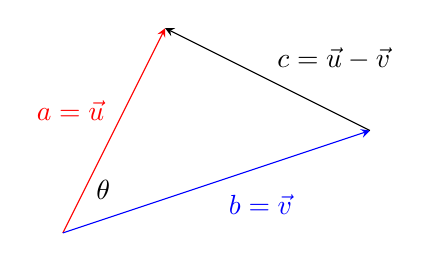
\begin{tikzpicture}[scale=1.3]
%\draw[help lines,step=1cm] (0,0) grid (3,2);
\draw[->,>=stealth,red] (0,0) -- node[above left ,fill=white] {$a=\norm{\vec u}$}(1,2);
\draw[->,>=stealth,blue] (0,0) -- node[below right=1pt,fill=white] {$b=\norm{\vec v}$} (3,1);
%\draw[<-,>=stealth,blue] [shift={(-2,1)}](0,0) -- node[above left=1pt,fill=white]{$-\vec v$} (3,1);
%\draw[->,>=stealth,ultra thick] (0,0) -- node[below left=0pt,fill=white] {$\vec u-\vec v$}(-2,1);
\draw[->,>=stealth,black] [shift={(3,1)}](0,0) -- node[above right=0pt,fill=white] {$c=\norm{\vec u-\vec v}$}(-2,1);
\draw(0,0) node[above right=3mm]{$\theta$};
\end{tikzpicture}
\end{center}
}}
Distributing on the left gives 
$$\vec u\cdot \vec u - 2 \vec u \cdot \vec v +\vec v\cdot \vec v = \vec u\cdot \vec u +\vec v\cdot \vec v -2\norm{\vec u}\norm{\vec v}\cos \theta.$$
Now cancel the common terms on both sides and divide by 2 to obtain our formula $\vec u \cdot \vec v = \norm{\vec u}\norm{\vec v}\cos \theta$.  
This formula geometrically explains how to connect the dot product to angles in both 2 and 3 dimensions.  
In higher dimensions, we can define the angle between two vectors using this formula.

If two vectors meet at a right angle, then since $\cos 90^\circ = 0$, we see that $\vec u \cdot \vec v = \norm{\vec u}\norm{\vec v}0=0$, so the dot product is zero. 
Similarly, if the dot product is zero, then $0=\vec u \cdot \vec v = \norm{\vec u}\norm{\vec v}\cos \theta$, so either one of the vectors has zero length or the angle between them is zero. 
We say that $\vec u$ and $\vec v$ are \define{orthogonal} if $\vec u \cdot \vec v=0$. 
\marginpar{orthogonal = dot product is zero}Two lines are perpendicular when the angle between then is $90^\circ$. Two vectors are orthogonal when either the angle between them is $90^\circ$ or one of the vectors is the zero vector.

\section{Multiplying Matrices}


\subsection{Linear Combinations}

\marginpar{The standard basis vectors in 3D:\\
$i = \vec \i = \left<1,0,0\right>=(1,0,0)$\\   
$j = \vec \j = \left<0,1,0\right>=(0,1,0)$\\ 
$k = \vec k = \left<0,0,1\right>=(0,0,1)$   
}The simplest vectors in 2D are (written in several different forms): 
$\ii = \vec \i = \left<1,0\right>=(1,0)$ and  
$\jj = \vec \j = \left<0,1\right>=(0,1)$. 
We call these the standard basis vectors in 2D. 
In 3D, we include the vector $\kk = \vec k=\left<0,0,1\right>$ as well as add a zero to both $\vec \i$ and $\vec \j$ to obtain the standard basis vectors. 

A similar idea is used in higher dimensions. 
The word \emph{basis} suggests that we can base other vectors on these basis vectors, and we typically write other vectors in terms of these standard basis vectors. 
Using only scalar multiplication and vector addition, we can obtain the other vectors in 2D from the standard basis vectors. 
For example, we can write $$\left<a,b\right> =a\left<1,0\right>+b\left<0,1\right> = a\vec\i+b\vec \j.$$ 
The entries of a row or column vector are called the coordinates of the vector relative to the standard basis, or just the components of the vector. 
Notice that we scaled the vectors $\vec \i$ and $\vec \j$, and then summed the scaled vectors. 
This is an example of a linear combination.

A \define{linear combination} of vectors $\vec v_{1}, \vec v_{2}, \ldots, \vec v_{n}$ is an expression of the form {$c_1\vec v_{1}+c_2\vec v_{2}+\ldots+c_n\vec v_{n}$}, where each {$c_i$} is a constant. 
A linear combination of vectors is simply a sum of scalar multiples of the vectors. 
We start with some vectors, stretch each one by some scalar, and then sum the result. 
Much of what we will do this semester, and in many applications of linear algebra to come, relates directly to understanding linear combinations.  

\begin{example}
Let's look at a physical application of linear combinations that you use every day when you drive.
When you place your foot on the accelerator of your car, the car exerts a force $\vec F_{1}$ pushing you forward. When you turn the steering wheel left, the car exerts a force $\vec F_{2}$ pushing you left. The total force acting on you is the vector sum of these forces, or a linear combination $\vec F_{\text{total}} = \vec F_1 +\vec F_2$. If $\vec T$ represents a unit vector pointing forward, and $\vec N$ represents a unit vector pointing left, then we can write the total force as the linear combination
$$\vec F_{\text{total}} = \norm{\vec F_1}\vec T +\norm{\vec F_2}\vec N.$$
To understand motion, we can now focus on finding just the magnitude of each force and the tangential unit vector $\vec T$ and normal unit vector $\vec N$.  Once we understand these quantities, we can understand any force because it is a linear combination of quantities we understand.
\end{example}

\subsection{Matrix Multiplication}

One of the key applications of linear combinations we will use throughout the semester is matrix multiplication. We will introduce the idea with an example.  
\begin{example}
Consider the three vectors 
$\begin{bmatrix}1\\0\\1\end{bmatrix}$,
$\begin{bmatrix}0\\2\\-3\end{bmatrix}$,
and 
$\begin{bmatrix}2\\1\\1\end{bmatrix}$.
Multiplying the first vector by $2$, the second by $-1$, the third by $4$, and then summing the result gives us the linear combination
$$2\begin{bmatrix}1\\0\\1\end{bmatrix}
-1\begin{bmatrix}0\\2\\-3\end{bmatrix}
+4\begin{bmatrix}2\\1\\1\end{bmatrix}
=
\begin{bmatrix}10\\2\\9\end{bmatrix} 
$$
We define matrix multiplication so that multiplying a matrix and a vector (with the vector on the right) corresponds precisely to creating a linear combination of the columns of $A$. 
The linear combination above in matrix form is
$$ 
\begin{bmatrix}1&0&2\\0&2&1\\1&-3&1\end{bmatrix}
\begin{bmatrix}2\\-1\\4\end{bmatrix}
=
\begin{bmatrix}10\\2\\9\end{bmatrix} 
.$$
\end{example}

\marginpar{Matrix multiplication $A\vec x$}
We define the matrix product $A\vec x$ (a matrix times a vector) to be the linear combination of columns of $A$ where the components of $\vec x$ are the scalars in the linear combination. 
For this to make sense, notice that the vector $\vec x$ must have the same number of entries as there are columns in $A$. 
Symbolically, let $\vec a_i$ be the $i$th column of $A$, so that 
$A = \begin{bmatrix}\vec a_1 & \vec a_2 &\cdots &\vec a_n\end{bmatrix}$, 
and let $\vec x = \begin{bmatrix}x_1\\x_2\\ \vdots \\ x_n\end{bmatrix}$. Then the matrix product is the linear combination 
\marginpar{The product $A\vec x$ gives us linear combinations of the columns of $A$.}
$$A\vec x 
=\begin{bmatrix}\vec a_1 & \vec a_2 &\cdots &\vec a_n\end{bmatrix}\begin{bmatrix}x_1\\x_2\\ \vdots \\ x_n\end{bmatrix}
= \vec a_1 x_1+\vec a_2 x_2+\cdots +\vec a_n x_n.$$ This should look like the dot product. If you think of $A$ as a ``vector'' of column vectors, then $A\vec x$ can be thought of as the dot product of $A$ and $\vec x$.  

\marginpar{Matrix multiplication $AB$}
We can now define the product of two matrices $A$ and $B$.  
Let $\vec b_j$ represent the $j$th column of $B$ (so $B = \begin{bmatrix}\vec b_1 & \vec b_2 &\cdots &\vec b_n\end{bmatrix}$).  The product $AB$ of two matrices {$A_{m\times n}$} and {$B_{n\times p}$} is a new matrix {$C_{m\times p}=[c_{ij}]$} where the $j$th column of $C$ is the product $A\vec b_j$.  To summarize, the matrix product $AB$ is a new matrix whose $j$th column is a linear combinations of the columns of $A$ using the entries of the $j$th column of $B$ to perform the linear combinations.  In math notation,\begin{equation*}
AB 
=A\begin{bmatrix}\vec b_1 & \vec b_2 &\cdots &\vec b_p\end{bmatrix}=\begin{bmatrix}A\vec b_1 & A\vec b_2 &\cdots & A\vec b_p\end{bmatrix}
\end{equation*}


\begin{example} 
In this example, the matrix $A$ has 3 rows, so the product should have 3 rows.  The matrix $B$ has 2 columns, so we need to find 2 different linear combinations giving us 2 columns in the product. 
$$ 
\begin{bmatrix}1 &2\\3&4\\5&6\end{bmatrix}
\begin{bmatrix}-2&0\\1&3\end{bmatrix} =
\begin{bmatrix}
\left(\begin{bmatrix}1\\3\\5\end{bmatrix}(-2)+\begin{bmatrix}2\\4\\6\end{bmatrix}(1)\right)
&
\left(\begin{bmatrix}1\\3\\5\end{bmatrix}(0)+\begin{bmatrix}2\\4\\6\end{bmatrix}(3)\right)
\end{bmatrix}
=
\begin{bmatrix}
\begin{matrix}0\\-2\\-4\end{matrix}&
\begin{matrix}6\\12\\18\end{matrix}
\end{bmatrix}$$
\end{example}



\begin{example} A row matrix times a column matrix is equivalent to the dot product of the two when treated as vectors.
$$ 
\begin{bmatrix}1 & 2\end{bmatrix}\begin{bmatrix}5\\6\end{bmatrix} =
\begin{bmatrix}1\cdot 5 + 2\cdot 6\end{bmatrix} = \begin{bmatrix}17\end{bmatrix}
$$
\end{example}



\begin{example} 
Note that $AB$ and $BA$ are usually different.
$$\begin{array}{cccc}
A=\begin{bmatrix} 1\\2\end{bmatrix}&
B=\begin{bmatrix} 3&4\end{bmatrix}&
AB= \begin{bmatrix} 3&4\\6&8\end{bmatrix} &
BA = [11]\end{array}
$$
Even if the product $CD$ is defined, the product $DC$ does not have to be.  In this example $D$ has 3 columns, but $C$ has only 2 rows, and hence the product $DC$ is not defined (as you can't form a linear combination of 3 vectors with only 2 constants).
$$
\begin{array}{cccc}
C =\begin{bmatrix} 1&2\\3&4\end{bmatrix}&
D =\begin{bmatrix} 0&1&-1\\1&0&2\end{bmatrix}&
CD =\begin{bmatrix} 2&1&3\\4&3&5\end{bmatrix}&
DC \text{ is undefined}
\end{array}$$
\end{example}

\marginpar{The identity matrix behaves like the number 1, in that $AI=IA=A$. 
\label{identity matrix}}The \define{identity matrix} is a square matrix which has only 1's along the diagonal, and zeros everywhere else. We often use $I_n$ to mean the $n$ by $n$ identity matrix. The identity matrix is like the number 1, in that $AI=A$ and $IA=A$ for any matrix $A$ of appropriate size.  If $A$ is a 2 by 3 matrix, then $AI_3=A$ and $I_2A=A$ (notice that the size of the identity matrix changes based on the order of multiplication).  If $A$ is a square matrix, then $AI=IA=A$.





\subsection{Alternate Definitions of Matrix Multiplication} 
Understanding matrix multiplication as linear combinations of vectors is very valuable (and we hope it is your first thought when you see matrix multiplication!)  There are many alternate ways to think of matrix multiplication. Here are two additional methods. Table \ref{matrixmult} illustrates all three.
\begin{description}
	\item[Row dot column.] The product {$AB$} of two matrices {$A_{m\times n}$} and {$B_{n\times p}$} is a new matrix {$C_{m\times p}=[c_{ij}]$} where $c_{ij}=\sum_{k=1}^n a_{ik}b_{kj}$ is the dot product of the of the {$i$}th row of {$A$} and the {$j$}th column of B.  Wikipedia has an excellent visual illustration of this approach.	
	 
	\item[Linear combinations of rows of $B$.] The matrix product $\vec x B$ (notice the vector is now on the left) is a linear combination of the rows of $B$ using the components of $\vec x$ as the scalars. For the product $AB$, let $\vec a_i$ represent the $i$th row of $A$.  Then the $i$th row of $AB$ is the product $\vec a_iB$, which is a linear combination of rows of $B$.  
\note{I'll eventually include a proof of why this works in the appendix.}
\end{description}

We'll use the ``linear combinations of columns'' view we first introduced because we eventually will want to think of a matrix $A$ as a function, and it is natural to write $A(\vec x)$ (with the vector on the right) to represent plugging the vector $\vec x$ into this function.

\begin{table}
\begin{tabular}{c}
Linear combinations of columns of $A$ with scalars from columns of $B$.
\\
\\
$ 
\begin{bmatrix}1 &2\\3&4\\5&6\end{bmatrix}
\begin{bmatrix}-2&0\\1&3\end{bmatrix} =
\begin{bmatrix}
\left(\begin{bmatrix}1\\3\\5\end{bmatrix}(-2)+\begin{bmatrix}2\\4\\6\end{bmatrix}(1)\right)
&
\left(\begin{bmatrix}1\\3\\5\end{bmatrix}(0)+\begin{bmatrix}2\\4\\6\end{bmatrix}(3)\right)
\end{bmatrix}
=
\begin{bmatrix}
\begin{matrix}0\\-2\\-4\end{matrix}&
\begin{matrix}6\\12\\18\end{matrix}
\end{bmatrix}$
\\\hline
\\
Rows of $A$ dotted by columns of $B$.
\\
\\
$ 
\begin{bmatrix}1 &2\\3&4\\5&6\end{bmatrix}
\begin{bmatrix}-2&0\\1&3\end{bmatrix} =
\begin{bmatrix}
\begin{matrix}
\begin{bmatrix}1&2\end{bmatrix}\begin{bmatrix}-2\\1\end{bmatrix}\\
\begin{bmatrix}3&4\end{bmatrix}\begin{bmatrix}-2\\1\end{bmatrix}\\
\begin{bmatrix}5&6\end{bmatrix}\begin{bmatrix}-2\\1\end{bmatrix}\\
\end{matrix}
&
\begin{matrix}
\begin{bmatrix}1&2\end{bmatrix}\begin{bmatrix}0\\3\end{bmatrix}\\
\begin{bmatrix}3&4\end{bmatrix}\begin{bmatrix}0\\3\end{bmatrix}\\
\begin{bmatrix}5&6\end{bmatrix}\begin{bmatrix}0\\3\end{bmatrix}\\
\end{matrix}
\end{bmatrix}
=
\begin{bmatrix}
\begin{matrix}0\\-2\\-4\end{matrix}&
\begin{matrix}6\\12\\18\end{matrix}
\end{bmatrix}$
\\\hline
\\
Use rows of $A$ to form linear combinations of rows of $B$.
\\\\
$
\begin{bmatrix}1 &2\\3&4\\5&6\end{bmatrix}
\begin{bmatrix}-2&0\\1&3\end{bmatrix} =
\begin{bmatrix}
1\begin{bmatrix}-2&0\end{bmatrix}+(2)\begin{bmatrix}1&3\end{bmatrix}
\\
3\begin{bmatrix}-2&0\end{bmatrix}+(4)\begin{bmatrix}1&3\end{bmatrix}
\\
5\begin{bmatrix}-2&0\end{bmatrix}+(6)\begin{bmatrix}1&3\end{bmatrix}
\end{bmatrix}
=
\begin{bmatrix}
\begin{matrix}0\\-2\\-4\end{matrix}&
\begin{matrix}6\\12\\18\end{matrix}
\end{bmatrix}$
\end{tabular}
\caption{Three ways to view matrix multiplication.\label{matrixmult}}\end{table}
















\section{Linear Systems of Equations}

A \define{linear system of equations}, such as 
$$\begin{array}{rl}
2x+y-z&=2\\
x-2y &=3\\
4y+2z&=1
\end{array}$$ is a system of equations where each variable in the system appears in its own term and is multiplied by a constant called a coefficient (which may be zero or one).  
Rather than using {$x,y,z$} as variables, we'll often use $x_1, x_2, x_3$, which allows us to easily extend to systems in higher dimensions. 
If we let $\vec v_i$ be a vector whose components are the constants next to $x_i$, then every linear system can be written in terms of linear combinations, i.e. $x_1\vec v_1+ x_2\vec v_2 + x_3\vec v_3=\vec b$. 
Similarly, we can write a linear system in terms of matrix multiplication $A\vec x = \vec b$, where the columns of $A$ are the vectors $\vec v_1, \vec v_2, \vec v_3$. 
The matrix $A$ is called the \definemargin{coefficient matrix} of the linear system of equations. 
Adding the column vector $\vec b$ to the right of $A$ gives what we call an \definemargin{augmented matrix} (where often a dashed or solid line is placed in the matrix to remind us of the equal sign). 
These four ways of representing a system are illustrated in Table \ref{systemequivalent}
\begin{table}
\begin{tabular}{cc}
 $x_1,x_2,x_3$ system& linear combination vector equation
\\\hline\hline
$\begin{array}{rl}
2x_1+x_2-x_3&=2\\
x_1-2x_2 &=3\\
4x_2+2x_3&=1
\end{array}$
&
$ x_1\begin{bmatrix}2\\1\\0\end{bmatrix} 
+ x_2\begin{bmatrix}1\\-2\\4\end{bmatrix} 
+ x_3\begin{bmatrix}-1\\0\\2\end{bmatrix} 
=\begin{bmatrix} 2\\3\\1\end{bmatrix} 
$
\\
\\
matrix equation & augmented matrix
\\\hline\hline
$ \begin{bmatrix}2&1&-1\\1&-2&0 \\0&4&2\end{bmatrix} 
\begin{bmatrix} x_{{1}}\\x_{{2}}\\x_{{3}}\end{bmatrix}
=\begin{bmatrix} 2\\3\\1\end{bmatrix} 
$
&
$\begin{bmatrix}[ccc|c]2&1&-1 &2\\1&-2&0 &3 \\0&4&2&1\end{bmatrix}$ 
\end{tabular}
\caption{Four equivalent ways to represent a system of equations.\label{systemequivalent}}
\end{table}

Let's add some geometry to the discussion. 
A linear equation in two variables $ax+by=c$ graphically represents a line.  
A system of equations with two variables represents multiple lines in the plane. 
A solution to such a system is a point that lies on all of the lines
(i.e., an intersection of all of the lines).
We can have one of the following situations:
\begin{enumerate}
\item No solution: no point lies on all of the lines (even if some of
  the lines intersect).
\item One solution: only one point lies on all the lines (i.e., all
  the lines intersect in one point).
\item Infinitely many solutions: the lines are actually all the same
  line, so all points on one line are really on all the lines.
\end{enumerate}

A linear equation in 3 variables $ax+by+cz=d$ represents a plane in space.  
In our 3D system above, a solution graphically represents the intersection of three planes. 
Three planes can intersect in any of the following ways:
\note{Add a picture here at some point}
\begin{enumerate}
\item No solution: two of the planes are parallel and never intersect,
  or the planes only intersect in pairs.
\item One solution: the three planes intersect in a single point.
\item Infinitely many solutions:
\begin{enumerate}
	\item the three planes all intersect in a line, so there is a line of solutions.
	\item the three equations all represent the same plane, so there is a plane of solutions.
\end{enumerate}
\end{enumerate}\note{TODO: make graphics of each of these situations.}
\marginpar{A system of equations will have either a unique solution, infinitely many solutions, or no solution.}%
In 2D and 3D, we can see geometrically that there will always be either
no solution, one solution, or infinitely many solutions.
With any system of linear equations, regardless of the number of equations and number of unknowns, this pattern continues. 
There will always be either no solution, a single solution, or infinitely many solutions.
Systems with solutions are called \define{consistent},
\marginpar{consistent system: has a solution}
whereas systems without solutions are called inconsistent.
%\marginpar{inconsistent}

A particularly important kind of linear system is of the form $A\vec x
= \vec 0$ (i.e., $\vec b=\vec 0$)---this kind of system is called a
\define{homogeneous} system.
\marginpar{homogeneous system: $A\vec x = \vec 0$}% 
If $A\vec x\neq \vec 0$ (i.e., $\vec b \neq \vec 0$), we say the
system is nonhomogeneous.  A homogeneous system is always consistent
since $\vec x=\vec 0$ is always a solution.  This solution is called
the \define{trivial solution}, and indicates that the graph of every equation
passes through the origin.  The big question for homogeneous systems
is whether they have nontrivial (nonzero) solutions.

\subsection{Gaussian Elimination}

Gaussian elimination is an efficient algorithm we will use to solve
systems of linear equations. This algorithm (or a variation) is commonly used
in practice.  The main idea is to eliminate each variable from all but
one equation/row (if possible), using the following three operations.
These operations are called \define{elementary row operations}.
\begin{enumerate}
  \item Multiply an equation (or row of a matrix) by a nonzero constant,
  \item Add a nonzero multiple of any equation (or row) to another equation,
  \item Interchange two equations (or rows).
\end{enumerate}
These three operations are the operations learned in college algebra
when solving a system using a method of elimination.  Gaussian
elimination is a way of organizing your work so that you always arrive
at a solution (or can determine there is no solution) in a certain
number of steps (that's part of the reason it is a good computer
algorithm). The process involves a forward reduction and (optionally)
a backward reduction. The forward reduction creates zeros in the lower
left corner of the matrix.  The backward reduction puts zeros in the
upper right corner of the matrix. We eliminate the values (i.e., make
them zero) in the lower left corner of the matrix, starting with
column 1, then column 2, and proceed column by column until all
values which can be eliminated have been
eliminated. Before formally stating the algorithm, let's look at a few
examples.

\begin{example}
Let's start with a system of 2 equations and 2 unknowns. The augmented
matrix representing the system is shown as well. To solve $$
\begin{array}{rr}
\begin{array}{rl}
x_1-3x_2&=4\\
2x_1-5x_2&=1 
\end{array}
&
\begin{bmatrix}[cc|c] 1&-3&4\\2&-5&1
\end{bmatrix} 
\end{array}
$$
we eliminate the $2x_1$ in the 2nd row by adding -2 times the first row to the second row.
$$\begin{array}{rr}
\begin{array}{rl}
x_1-3x_2&=4\\
x_2&=-7 
\end{array}
&
\begin{bmatrix}[cc|c] 1&-3&4\\0&1&-7
\end{bmatrix} 
\end{array}
$$
Now the augmented matrix is said to be in \definemargin{row echelon form}. This means that 
\begin{itemize}
	\item in each nonzero row, the first nonzero entry is a 1 (called a ``leading 1''),
  \item the leading 1 in a row occurs further right than the leading 1 in the row above, and
  \item any rows of all zeros appear at the bottom.
\end{itemize}
The position in the matrix where the leading 1 occurs is called a pivot. 
The column containing a pivot is called a \definemargin{pivot column}. 
At this point we can use ``back-substitution'' to get {$x_2=-7$} and {$x_1=4+3x_2 = 4-21=-17$}. 
Alternatively, we can continue the elimination process by eliminating
the terms above each pivot, starting with the rightmost (and lowest) pivot and
working towards the left and top.
This will result in a matrix where the only nonzero entry in any pivot column is the pivot entry (i.e., the leading 1). 
In our example, if we add 3 times the second row to the first row, we obtain
$$\begin{array}{rr}
\begin{array}{rl}
x_1&=-17\\
x_2&=-7 
\end{array}
&
\begin{bmatrix}[cc|c] 1&0&-17\\0&1&-7
\end{bmatrix} 
\end{array}
$$
The matrix on the right is said to be in \define{reduced row echelon form} (or just ``rref''). 
\marginpar{rref=reduced row echelon form}%
A matrix is in reduced row echelon form if 
\begin{itemize}
	\item the matrix is in echelon form, and 
	\item the only nonzero entry in each pivot column is the pivot entry (i.e., the leading 1).
\end{itemize}
 You can easily read solutions to systems of equations directly from a matrix which is in reduced row echelon form.

We can interpret the solution $x_1=-17$, $x_2=-7$ in multiple ways.  It is the point $(-17,-7)$ where the two lines $x-3y=4$ and $
2x-5y=1$ intersect.  We also know that the only way to obtain a solution to the vector equation 
$c_1
\begin{bmatrix}
1\\
2
\end{bmatrix}
+
c_2
\begin{bmatrix}
-3\\
-5
\end{bmatrix}
=
\begin{bmatrix}
4\\
1
\end{bmatrix}
$ is to let $c_1=-17$ and $c_2=-7$, which shows us that $(4,1)$ is a linear combination of the vectors $(1,2)$ and $(-3,-5)$.  In addition, the only solution to the matrix equation 
$\begin{bmatrix}1&-3\\ 2 &-5 \end{bmatrix}\begin{bmatrix}x_1\\ x_2\end{bmatrix}=\begin{bmatrix}4\\1\end{bmatrix}$ 
is 
$\begin{bmatrix}x_1\\x_2\end{bmatrix}=\begin{bmatrix}-17\\-7\end{bmatrix}$.  \marginpar{Row reduction helps us understand systems, vector equations, and matrix equations.} Notice that solving this system of equations tells us information about graphical intersections, linear combination of vectors, and matrix equations.
\end{example}


\begin{example}
Let's now solve a nonhomogeneous (meaning the right side is not zero) system with 3 equations and 3 unknowns: $$\begin{array}{rl}
2x_1+x_2-x_3&=2\\
x_1-2x_2 &=3\\
4x_2+2x_3&=1
\end{array} \quad\quad\quad\quad\quad
\begin{bmatrix}[ccc|c] 2&1&-1&2\\1&-2&0&3\\0&4&2&1\end{bmatrix}.$$
We'll encounter some homogeneous systems later on.  To simplify the
writing, we'll just use matrices this time.  To keep track of each
step, we will write the row operation next to the row we will replace.
Remember that the three operations are (1) multiply a row by a nonzero
constant, (2) add a multiple of one row to another, and (3)
interchange any two rows.  If we write $R_2+3R1$ next to $R_2$, then
this means we will add 3 times row 1 to row 2.  If we write $2R_2-R1$
next to $R_2$, then we have done two row operations, namely we
multiplied $R_2$ by $2$, and then added $(-1)$ times $R1$ to the result
(replacing $R2$ with the sum).  The steps below read left to right,
top to bottom.  In order to avoid fractions in the middle of the
computation, we wait to divide each pivot entry to make it a 1 until
the last step.
$$\begin{array}{rlcl}
\Rightarrow^{(1)}&
 \begin{bmatrix}[ccc|c] 2&1&-1&2\\1&-2&0&3\\0&4&2&1\end{bmatrix}
  \begin{array}{lr} \ \\2R_2-R_1\\ \ \end{array}
&\Rightarrow^{(2)}& 
\begin{bmatrix}[ccc|c] 2&1&-1&2\\0&-5&1&4\\0&4&2&1\end{bmatrix} 
\begin{array}{lr}\ \\ \ \\5R_3+4R_2 \end{array}
\\ \\ \Rightarrow^{(3)}&
 \begin{bmatrix}[ccc|c] 2&1&-1&2\\0&-5&1&4\\0&0&14&21\end{bmatrix} 
 \begin{array}{lr}\ \\ \ \\R_3/7 \end{array}
&\Rightarrow^{(4)}& 
\begin{bmatrix}[ccc|c] 2&1&-1&2\\0&-10&2&8\\0&0&2&3\end{bmatrix} 
\begin{array}{l} 2R_1+R_3\\R_2-R_3\\ \ \end{array}
\\ \\ \Rightarrow^{(5)}&
 \begin{bmatrix}[ccc|c] 4&2&0&7\\0&-10&0&5\\0&0&2&3\end{bmatrix}  
 \begin{array}{lr}\ \\R_2/5\\ \ \end{array} 
&\Rightarrow^{(6)}& 
\begin{bmatrix}[ccc|c] 4&2&0&7\\0&-2&0&1\\0&0&2&3\end{bmatrix}  
\begin{array}{lr} R_1+R_2\\ \ \\ \ \end{array}
\\ \\ \Rightarrow^{(7)}&
\begin{bmatrix}[ccc|c] 4&0&0&8\\0&-2&0&1\\0&0&2&3\end{bmatrix} 
\begin{array}{lr} R_1/4\\R_2/-2\\R_3/2 \end{array}
&\Rightarrow^{(8)}&  
\begin{bmatrix}[ccc|c] 1&0&0&2\\0&1&0&-1/2\\0&0&1&3/2\end{bmatrix} 
\end{array}
$$
Writing the final matrix in terms of a system of linear equations, we have the solution {$x_1=2$, $x_2=-1/2$, $x_3=3/2$}. Remember that this tells us (1) where three planes intersect, (2) how to write the 4th column $\vec b$ in our original augmented matrix as a linear combination of the columns of the coefficient matrix $A$, and (3) how to solve the matrix equation $A\vec x = \vec b$ for $\vec x$.
\end{example}


The following steps describe the Gaussian elimination algorithm that we used above. 
Please take a moment to compare what is written below with the example above. 
Most of the problems in this unit can be solved using Gaussian elimination, so we will practice it as we learn a few new ideas.  

A key idea in Gaussian elimination is that we methodically eliminate entries in the matrix (by making them zero) in such a way that the entries we make zero will stay zero throughout the rest of the computation.
\begin{enumerate}
\item Forward Phase (getting row echelon form): the following 4 steps should be repeated until you have mentally erased all the rows or all the columns. In step 1 or 4, you will erase a column and/or row from the matrix.
\begin{enumerate}
	\item
	\marginpar{Computer algorithms often place the largest (in absolute value) nonzero entry in the first row. This reduces potential errors due to rounding that can occur in later steps.}%
Consider the first column of your matrix. Start by interchanging rows (if needed) to place a nonzero entry in the first row. If all the elements in the first column are zero, then ignore that column in future computations (mentally erase the column) and begin again with the smaller matrix which is missing this column. If you erase the last column, then stop.
  \item 
  Divide the first row (of your possibly smaller matrix) by its leading entry so that you have a leading 1. This entry is a pivot, and the column is a pivot column. 
	\item Use the pivot to eliminate each nonzero entry below the pivot by adding a multiple of the row with the pivot to the nonzero lower row.
	\item 
	\marginpar{Ignoring rows and columns is equivalent to incrementing row and column counters in a computer program.}%
	Ignore the row and column containing your new pivot and return to the first step (mentally cover up or erase the row and column containing your pivot). If you erase the last row, then stop.
\end{enumerate}
	\item Backward Phase (getting reduced row echelon form): at this point, any row that has a nonzero entry should start with a leading~1 (the pivot for the row), and you should have all zeros to the left and below each leading~1.
\begin{enumerate}
	\item Start with the last pivot column.   Use the pivot in that column to eliminate all the nonzero entries above it by adding multiples of the row containing the pivot to the nonzero rows above. 
	\item Work from right to left, using each pivot in turn to eliminate the nonzero entries above it. Nothing to the left of the current pivot column will change in an elimination step.  By working right to left, you methodically work through the matrix and greatly reduce the number of computations needed to fully reduce the matrix.
\end{enumerate}
\end{enumerate}

When doing row reduction by hand, it is often convenient to skip step 1(b) initially to avoid arithmetic involving fractions. Instead of making the first entry in the row a one, you can also find a common multiple of all the terms in the row and divide by the common mulitple to reduce the size of the numbers in the row.  If you skip 1(b) initially, then at the start of the backward phase, the pivot entries may not all be ones.  In this case, after finishing the backward phase, you should divide all the rows by their first nonzero entry in order to make each pivot entry a one.

To summarize, first we work from left to right and use pivot entries to eliminate (make zero) all the entries below the pivots.  Then we work right to left and use the pivot entries to eliminate all entries above the pivots.

\begin{example}\label{ex rref last}
As a final example, let's reduce 
{\small $
\begin{bmatrix}[cccc|c]
 0 & 1 & 1 & -2 & 7 \\
  1 & 3 & 5 & 1 & 6 \\
 2 & 0 & 4 & 3 & -8 \\
 -2 & 1 & -3 & 0 & 5
\end{bmatrix}
$} to reduced row echelon form (rref). The first step involves swapping two rows. We swap row 1 and row 2 because this places a 1 as the leading entry in row 1.
{\small  $$\begin{array}{rlcl}
\multicolumn{2}{l}{\text{(1) Get a nonzero entry in upper left}}&
\multicolumn{2}{l}{\text{(2) Eliminate entries in 1st column}}\\
\Rightarrow&
\begin{bmatrix}[cccc|c]
 0 & 1 & 1 & -2 & 7 \\
  1 & 3 & 5 & 1 & 6 \\
 2 & 0 & 4 & 3 & -8 \\
 -2 & 1 & -3 & 0 & 5
\end{bmatrix}
  \begin{array}{lr} R_1\leftrightarrow R_2 \\ \ \\ \ \\ \ \end{array}
&\Rightarrow& 
\begin{bmatrix}[cccc|c]
  1 & 3 & 5 & 1 & 6 \\
 0 & 1 & 1 & -2 & 7 \\
 2 & 0 & 4 & 3 & -8 \\
 -2 & 1 & -3 & 0 & 5
\end{bmatrix}
  \begin{array}{lr} \ \\ \ \\ R_3-2R_1 \\ R_4+2R_1 \end{array}
\\ \\
\multicolumn{2}{l}{\text{(3) Eliminate entries in 2nd column}}&
\multicolumn{2}{l}{\text{(4) Make a leading 1 in 4th column}}\\
\Rightarrow&
\begin{bmatrix}[cccc|c]
  1 & 3 & 5 & 1 & 6 \\
 0 & 1 & 1 & -2 & 7 \\
 0 & -6 & -6 & 1 & -20 \\
 0 & 7 & 7 & 2 & 17
\end{bmatrix}
  \begin{array}{lr} \ \\ \ \\ R_3+6R_2 \\ R_4-7R_2 \end{array}
&\Rightarrow& 
\begin{bmatrix}[cccc|c]
  1 & 3 & 5 & 1 & 6 \\
 0 & 1 & 1 & -2 & 7 \\
 0 & 0 & 0 & -11 & 22 \\
 0 & 0 & 0 & 16 & -32
\end{bmatrix}
  \begin{array}{lr} \ \\ \ \\ R_3/(-11) \\ R_4/16 \end{array}
\\ \\
\multicolumn{2}{l}{\text{(5) Eliminate entries in 4th column}}&
\multicolumn{2}{l}{\text{(6) Row Echelon Form}}\\
\Rightarrow&
\begin{bmatrix}[cccc|c]
  1 & 3 & 5 & 1 & 6 \\
 0 & 1 & 1 & -2 & 7 \\
 0 & 0 & 0 & 1 & -2 \\
 0 & 0 & 0 & 1 & -2
\end{bmatrix}
  \begin{array}{lr} \ \\ \ \\ \ \\ R_4-R_3 \end{array}
&\Rightarrow& 
\begin{bmatrix}[cccc|c]
  1 & 3 & 5 & 1 & 6 \\
 0 & 1 & 1 & -2 & 7 \\
 0 & 0 & 0 & 1 & -2 \\
 0 & 0 & 0 & 0 & 0
\end{bmatrix}
\end{array}
$$}\begin{picture}(0,0)

\begin{tikzpicture}[scale=.39]
\draw[help lines,step=1cm,transparent] (0,0) grid (30,20);
\draw[opacity=.2,fill][shift={(2.6,16.6)}] (0,0) rectangle (1.4,.8);
\draw[opacity=.2,fill][shift={(19.6,13.6)}] (0,0) rectangle (1.4,2.8);
\draw[opacity=.1,fill][shift={(2.6,10.6)}] (0,0) rectangle (8.9,.8);
\draw[opacity=.1,fill][shift={(2.6,7.6)}] (0,0) rectangle (.7,3.8);
\draw[opacity=.2,fill][shift={(3.9,7.6)}] (0,0) rectangle (1.4,1.8);
\draw[opacity=.1,fill][shift={(19.5,10.6)}] (0,0) rectangle (8.1,.8);
\draw[opacity=.1,fill][shift={(19.5,7.6)}] (0,0) rectangle (.7,3.8);
\draw[opacity=.1,fill][shift={(20.8,9.6)}] (0,0) rectangle (6.8,.8);
\draw[opacity=.1,fill][shift={(20.8,7.6)}] (0,0) rectangle (.7,2.8);
\draw[opacity=.1,fill][shift={(22.15,7.6)}] (0,0) rectangle (.7,1.8);
\draw[opacity=.2,fill][shift={(23.6,8.6)}] (0,0) rectangle (1.6,.8);

\draw[opacity=.1,fill][shift={(2.6,4.6)}] (0,0) rectangle (7.2,.8);
\draw[opacity=.1,fill][shift={(2.6,1.6)}] (0,0) rectangle (.7,3.8);
\draw[opacity=.1,fill][shift={(3.9,3.6)}] (0,0) rectangle (5.9,.8);
\draw[opacity=.1,fill][shift={(3.9,1.6)}] (0,0) rectangle (.7,2.8);
\draw[opacity=.1,fill][shift={(5.2,1.6)}] (0,0) rectangle (.7,1.8);
\draw[opacity=.2,fill][shift={(6.7,1.6)}] (0,0) rectangle (1.1,.8);

\draw[opacity=.1,fill][shift={(19.5,4.6)}] (0,0) rectangle (7.2,.8);
\draw[opacity=.1,fill][shift={(19.5,1.6)}] (0,0) rectangle (.7,3.8);
\draw[opacity=.1,fill][shift={(20.8,3.6)}] (0,0) rectangle (5.9,.8);
\draw[opacity=.1,fill][shift={(20.8,1.6)}] (0,0) rectangle (.7,2.8);
\draw[opacity=.1,fill][shift={(22.15,1.6)}] (0,0) rectangle (.7,1.8);
\draw[opacity=.1,fill][shift={(23.6,1.6)}] (0,0) rectangle (1.1,1.8);
\draw[opacity=.1,fill][shift={(23.6,2.6)}] (0,0) rectangle (3.1,.8);
\draw[opacity=.1,fill][shift={(25.6,1.6)}] (0,0) rectangle (1.1,.8);

\end{tikzpicture}
\end{picture}At this stage, we have found a row echelon form of the matrix. 
Notice that we eliminated nonzero terms in the lower left of the matrix by starting with the first column and working our way to the right column by column.  Columns 1, 2, and 4 are the pivot columns of this matrix. We now use the pivots to eliminate the other nonzero entries in each pivot column (working right to left).\marginpar{Recall that a matrix is in reduced row echelon (rref) if:
\begin{enumerate}
	\item Nonzero rows begin with a leading 1. 
	\item Leadings 1's on subsequent rows appear further right than previous rows. 
	\item Rows of zeros are at the bottom.
	\item Zeros are above and below each pivot.
\end{enumerate}}
{\small $$ \begin{array}{rlcl}
\multicolumn{2}{l}{\text{(7) Eliminate entries in 4th column}}&
\multicolumn{2}{l}{\text{(8) Eliminate entries in 2nd column}}\\
\Rightarrow&
\begin{bmatrix}[cccc|c]
  1 & 3 & 5 & 1 & 6 \\
 0 & 1 & 1 & \begin{picture}(0,0)(0,3) \tikz \draw[scale=.39,fill,opacity=.2] (0,0) rectangle (1.6,2);\end{picture}
							-2 & 7 \\
 0 & 0 & 0 & 1 & -2 \\
 0 & 0 & 0 & 0 & 0
\end{bmatrix}
  \begin{array}{lr} R_1-R3 \\ R_2+2R_3 \\ \ \\ \ \end{array}
&\Rightarrow& 
\begin{bmatrix}[cccc|c]
  1 & \begin{picture}(0,0)(4,3) \tikz \draw[scale=.39,fill,opacity=.2] (0,0) rectangle (1,1);\end{picture}
  		3 & 5 & 0 & 8 \\
 0 & 1 & 1 & 0 & 3 \\
 0 & 0 & 0 & 1 & -2 \\
 0 & 0 & 0 & 0 & 0
\end{bmatrix}
  \begin{array}{lr} R_1-3R_2 \\ \ \\ \ \\ \ \end{array}
\\ \\ 
\multicolumn{2}{l}{\text{(9) Reduced Row Echelon Form}}&
\multicolumn{2}{l}{\text{(10) Switch to system form}}\\
\Rightarrow&
\begin{bmatrix}[cccc|c]
  1 & 0 & 2 & 0 & -1 \\
 0 & 1 & 1 & 0 & 3 \\
 0 & 0 & 0 & 1 & -2 \\
 0 & 0 & 0 & 0 & 0
\end{bmatrix}
&\Rightarrow& 
\begin{array}{rl}
x_1+2x_3&=-1\\
x_2+x_3&=3\\
x_4&=-2\\
0&=0
\end{array}
\end{array}
$$}We have obtained the reduced row echelon form. 
When we write this matrix in the corresponding system form, notice that there is not a unique solution to the system. Because the third column did not contain a pivot column, we can write every variable in terms of $x_3$ (the redundant equation $x_3=x_3$ allows us to write $x_3$ in terms of $x_3$). We are free to pick any value we want for $x_3$ and still obtain a solution. For this reason, we call $x_3$ a \define{free variable}, \marginpar{Free variables correspond to non pivot columns. Solutions can be written in terms of free variables.} and write our infinitely many solutions in terms of $x_3$ as 
$$
\begin{array}{ll}
x_1=-1-2x_3\\
x_2=3-x_3\\
x_3=x_3\\
x_4=-2
\end{array}
\quad \text{ or by letting $x_3=t$, }\quad
\begin{array}{ll}
x_1=-1-2t\\
x_2=3-t\\
x_3=t\\
x_4=-2
\end{array}
.
$$
\marginpar{parametric form}By choosing a value (such as $t$) for $x_3$, we can write our solution in what we call ``parametric form.'' We have now given a parametrization of the solution set, where $t$ is an arbitrary real number.  We can also write the solution in vector form: $\vec x=\left<x_1,x_2,x_3,x_4\right>=\left< -1-2t, 3-t, t, -2\right>$, where $-\infty<t<\infty$. 
\end{example}

\subsection{Reading Reduced Row Echelon Form (``rref'')}

From reduced row echelon form, you can read the solution to a system immediately from the augmented matrix.  Here are some typical examples of what you will see when you reduce an augmented matrix which represents a system that does not have a unique solution. The explanations which follow illustrate how to see the solution immediately from the matrix.
$$\begin{array}{ccc}
 \begin{bmatrix}[ccc|c] 1&2&0&1\\0&0&1&3
\\0&0&0&0\end{bmatrix} 
& \begin{bmatrix}[ccc|c] 1&0&4&-5\\0&1&-2&3
\end{bmatrix} 
& \begin{bmatrix}[ccc|c] 1&0&2&0\\0&1&-3&0
\\0&0&0&1\end{bmatrix} 
\\
\vec x = \left<1-2x_2,x_2,3\right>
&\vec x = \left<-5-4x_3,3+2x_3,x_3\right>
&\text{no solution since } 0\neq1
\end{array}
$$

\begin{example}
In the first example, columns 1 and 3 are the pivot columns. Since column 2 is not a pivot column, we'll let $x_2$ be a free variable and write the solution in terms of $x_2$. Rewriting the first matrix in system form yields $x_1+2x_2 =1,x_3=3$, or solving for each variable in terms of $x_2$, we have $x_1=1-x_2,x_3=3$.  
Adding to this system the redundant equation $x_2=x_2$, we have in vector form 
$\begin{bmatrix}x_1\\x_2\\x_3\end{bmatrix} = \begin{bmatrix}1-2x_2\\x_2\\3\end{bmatrix} = \begin{bmatrix}1\\0\\3\end{bmatrix} + x_2 \begin{bmatrix}-2\\1\\0\end{bmatrix}$. 
Sometimes it's useful to use a different variable, such as $x_2=t$, and then write the solution in parametric form as $\left<x_1,x_2,x_3\right>=\left<1-2t,t,3\right>$, where $t$ is any real number. This solution is a line in space. \note{a picture would be nice---maybe in the Sage version of the text?}
\end{example}

\begin{example}
In the second example, the first and second columns are pivot columns, so $x_3$ is a free variable.  The solution can be written in the form 
$\begin{bmatrix}x_1\\x_2\\x_3\end{bmatrix} = \begin{bmatrix}-5-4x_3\\3+2x_3\\x_3\end{bmatrix} = \begin{bmatrix}-5\\3\\0\end{bmatrix} + x_3 \begin{bmatrix}-4\\2\\1\end{bmatrix}$.  Notice that the third and fourth columns of the matrix appear as parts of the vectors in the solution.
\end{example}

\begin{example}
In the third example, the first, second, and fourth columns are pivot columns. Because the last column is a pivot column, we obtain the equation $0=1$, which is absurd.  Hence the system is inconsistent and has no solution.
\end{example}

\begin{example}
The ideas above generalize to higher dimensions. Here are two large rref matrices and their solutions.

\begin{center}
\begin{tabular}{cc}
$\begin{bmatrix}[ccccc|c] 0&1&0&2&0&0\\0&0&1&3&0&1\\0&0&0&0&1&4\\0&0&0&0&0&0\end{bmatrix}$
&
$\begin{bmatrix}x_1\\x_2\\x_3\\x_4\\x_5\end{bmatrix} 
= \begin{bmatrix}0\\0\\1\\0\\4\end{bmatrix}
+x_1\begin{bmatrix}1\\0\\0\\0\\0\end{bmatrix}
+x_4\begin{bmatrix}0\\-2\\-3\\1\\0\end{bmatrix}$
\\
$\begin{bmatrix}[cccccc|c] 0&1&0&2&0&0&0\\0&0&1&3&0&1&0\\0&0&0&0&1&4&0\\0&0&0&0&0&0&0\end{bmatrix}$
&
$\begin{bmatrix}x_1\\x_2\\x_3\\x_4\\x_5\\x_6\end{bmatrix} 
= \begin{bmatrix}0\\0\\0\\0\\0\\0\end{bmatrix}
+x_1\begin{bmatrix}1\\0\\0\\0\\0\\0\end{bmatrix}
+x_4\begin{bmatrix}0\\-2\\-3\\1\\0\\0\end{bmatrix}
+x_6\begin{bmatrix}0\\0\\-1\\0\\-4\\1\end{bmatrix}$
\end{tabular}
\end{center}
Each non-pivot column corresponds to one of the vectors in the sum above.  
\end{example}









\section{Rank and Linear Independence}

The \define{rank} of a matrix is the number of pivot columns of the matrix. To find the rank of a matrix, reduce the matrix using Gaussian elimination until you discover the pivot columns (you only need to do the forward phase for this).

Recall that a linear combination of vectors {$\vec v_{1},\vec v_{2},\ldots,\vec v_{n}$} is an expression of the form {$c_1\vec v_{1}+c_2\vec v_{2}+\ldots+c_n\vec v_{n}$}, where {$c_i$} is a constant scalar for each $i$. 
A linear combination of vectors is a sum of scalar multiples of the vectors. 
Also recall that a linear combination of vectors is really just matrix multiplication, $A\vec c$, where the columns of $A$ are the vectors $\vec v_i$ and $\vec c= \left<c_1,c_2,\ldots,c_n\right>$. We will try to emphasis this in what follows.

First we need another definition. The \definemargin{span} of a set of vectors is the set of all possible linear combinations of the vectors.  We often write this as $\vspan\{\vec v_1, \vec v_2, \ldots, \vec v_n\}$.  In terms of matrices, if $A$ is the matrix with columns $\vec v_1, \vec v_2, \ldots, \vec v_n$, then the span of $\vec v_1, \vec v_2, \ldots, \vec v_n$ is the set of all possible vectors $\vec b$ such that $A\vec x=\vec b$ for some $\vec x$.

\begin{example}\label{ex span}
\begin{enumerate}
	\item The span of the vector $\left<1,0,0\right>$ is the set of vectors of the form $a\left<1,0,0\right> = \left<a,0,0\right>$, which is the $x$-axis, a line through the origin. 
	\item The span of the vectors $\left<1,0,0\right>$ and $\left<0,1,0\right>$ is the set of vectors in 3D of the form $a\left<1,0,0\right>+b\left<0,1,0\right>=\left<a,b,0\right>$, which is the $xy$-plane, a plane through the origin. 
	\item The span of $\left<2,0,1\right>$ and $\left<-1,-2,3\right>$ is the set of vectors 
	$$a\langle 2,0,1\rangle+b\langle-1,-2,3\rangle
		= \langle2a-b,-2b,a+3b\rangle
		= \begin{bmatrix} \cl{2\\0\\1}&\cl{-1\\-2\\3}\end{bmatrix}
	\begin{bmatrix}a\\b\end{bmatrix} 
	=\begin{bmatrix}2a-b\\-2b\\a+3b\end{bmatrix}.$$
        This is again a plane in 3D that passes through the origin.
\end{enumerate}
\end{example}
Geometrically you can obtain the span of vectors by adding together all possible stretches of the given vectors. The span of a set of vectors will be a line, a plane, or some higher-dimensional version of these objects (called a hyperplane) which passes through the origin. 

We say that a set of vectors is \definemargin{linearly independent} if the only solution to the homogeneous system $c_1\vec v_{1}+c_2\vec v_{2}+\ldots+c_n\vec v_{n}=\vec 0$ is the trivial solution $c_1=c_2=\cdots=c_n=0$. 
Otherwise we say the set of vectors is linearly dependent, since one of the vectors depends on (can be obtained as a linear combination of) the others. In terms of spans, we say a set of vectors is linearly dependent when one of the vectors is in the span of the other vectors. 

\begin{example}\label{first linearly independent example}
The set $\{\langle1,0\rangle, \langle0,1\rangle\}$ is linearly independent, whereas the set $\{\langle2,4\rangle, \langle3,6\rangle\}$ is linearly dependent (notice that $\langle3,6\rangle = \frac{3}{2}\langle2,4\rangle$ is a linear combination of $\langle2,4\rangle$). The set $\{\langle1,2,0\rangle, \langle2,0,3\rangle, \langle3,-2,6\rangle\}$ is linearly dependent because there is a nonzero linear combination of the three vectors that yields the zero vector:
$$-1\langle1,2,0\rangle+2\langle2,0,3\rangle-1\langle3,-2,6\rangle=\langle0,0,0\rangle.$$ 
Alternatively, we know the vectors are dependent because we can write the third vector as a linear combination of the first two:
$${\color{blue}-1}\langle1,2,0\rangle+{\color{red}2}\langle2,0,3\rangle=\langle3,-2,6\rangle.$$ 
To find this linear combination, we write the first linear combination as a homogeneous system (in matrix form) $A\vec c=\vec 0$:  
\marginpar{When solving a homogeneous system of equations, the column of zeros at the right contributes no new information, and so is often omitted.}
$$\begin{bmatrix}
\cl{1\\2\\0}
&\cl{2\\0\\3}
&\cl{3\\-2\\6}
\end{bmatrix}
\begin{bmatrix}
c_1\\c_2\\c_3
\end{bmatrix}
=
\begin{bmatrix}
0\\0\\0
\end{bmatrix}
\quad\quad\quad
\begin{bmatrix}[ccc|c]
\cl{1\\2\\0}
&\cl{2\\0\\3}
&\cl{3\\-2\\6}
&\cl{0\\0\\0}
\end{bmatrix}
\xrightarrow{\rref}
\begin{bmatrix}[ccc|c]
\cl{1\\0\\0}
&\cl{0\\1\\0}
&\cl{{\color{blue}-1}\\{\color{red}2}\\0}
&\cl{0\\0\\0}
\end{bmatrix}
$$
The reduced row echelon form tells us that column 3 is not a pivot column.  This is precisely why the third column can be written as a linear combination of the first two, and the numbers in column 3 tell us precisely what coefficients ($-1$ and $2$) to use writing the third column as a linear combination of the pivot columns. 
\end{example}

An easy way to test if vectors are linearly independent is to create a matrix $A$ where each column represents one of the vectors. 
The vectors are linearly independent if the only solution to $A\vec c=\vec 0$ is $\vec c=0$. Row reduce the matrix to reduced row echelon form. 
The vectors are linearly independent if and only if each column of $A$ is a pivot column (which forces $\vec c$ to be zero). 
If a column is not a pivot column, then the vector corresponding to that column can be written as a linear combination of the preceding vectors using the coefficients in that column. 

\begin{example}
The vectors 
$[1\ 3\ 5]$,
$[-1\ 0\ 1]$, and
$[0\ 3\ 1]$ 
are linearly independent, as the reduced row echelon form of 
$ \begin{bmatrix} 1&-1&0\\3&0&3\\5&1&1\end{bmatrix}$ is 
$ \begin{bmatrix} 1&0&0\\0&1&0\\0&0&1\end{bmatrix}$, 
and each column is a pivot column.
\end{example}
\begin{example}
The vectors $[1\ 3\ 5]$, 
$[-1\ 0\ 1]$, and $[1\ 6\ 11]$
%$
% \begin{bmatrix} 1&3&5\end{bmatrix}
%\begin{bmatrix} -1&0&1\end{bmatrix}
% \begin{bmatrix} 1&6&11\end{bmatrix} 
%$ 
are linearly dependent, as the reduced row echelon form of 
$ \begin{bmatrix} 1&-1&1\\3&0&6\\5&1&11\end{bmatrix} $ 
is 
$ \begin{bmatrix} 1&0&2\\0&1&1\\0&0&0\end{bmatrix}$, 
and column 3 is not a pivot column. This immediately means that the third vector (of the original matrix) is a linear combination of the preceding two. Using the coefficients 2 and 1 from the third column, we can write 
$[1\ 6\ 11] = 2 [1\ 3\ 5]+1[-1\ 0\ 1]$. 
\end{example}
In the preceding example, the coefficients in the linear combination (2 and 1) are called the \definemargin{coordinates} of $[1~6~11]$ relative to the vectors $[1~3~5]$ and $[-1~0~1]$.  We could write down the linear combination because the third column of the matrix, $[1~6~11]$, was not a pivot column.  Notice that we could have read the coordinates right out of the third column of the rref matrix.  Every non-pivot column of a matrix can be expressed as a linear combination of the pivot columns, where the coordinates of the non-pivot column come from the same non-pivot column in the rref matrix.


We have used the concept of \textit{coordinates of a vector relative to other vectors} to state that the coordinates of $(2,-3,4)$ relative to $(1,0,0),(0,1,0),(0,0,1)$ are  $2$, $-3$, and $4$.  We will study this concept of coordinates in greater depth later.

\subsection{Linear Combinations, Spans, and RREF}
Solving a system of equations such as $x+3y=0$, $2x-y=5$ is equivalent to solving the vector equation 
$x\begin{bmatrix} 1\\2\end{bmatrix}+y\begin{bmatrix} 3\\-1\end{bmatrix}=\begin{bmatrix} 0\\5\end{bmatrix}$. This is also equivalent to the following questions.
\begin{itemize}
	\item Is $\begin{bmatrix} 0\\5\end{bmatrix}$ a linear combination of the vectors $\begin{bmatrix} 1\\2\end{bmatrix}$ and $\begin{bmatrix} 3\\-1\end{bmatrix}$?
	\item Is $\begin{bmatrix} 0\\5\end{bmatrix}$ in the span of $\begin{bmatrix} 1\\2\end{bmatrix}$ and $\begin{bmatrix} 3\\-1\end{bmatrix}$?
\end{itemize}
To answer all these questions, first reduce the matrix $\begin{bmatrix}[cc|c]1&3& 0\\2&-1&5\end{bmatrix}$ to reduced row echelon form.
\begin{align*}
   &\begin{bmatrix}[cc|c]1&3& 0\\2&-1&5\end{bmatrix}\begin{array}{l}\\ R_2-2R_1\end{array}
 \Rightarrow 
   \begin{bmatrix}[cc|c]1&3& 0\\0&-7&5\end{bmatrix} \begin{array}{l} 3R_2+7R_1\\ \ \end{array}\\
 \Rightarrow 
   &\begin{bmatrix}[cc|c]7&0& 15\\0&-7&5\end{bmatrix} \begin{array}{l}R_1/7\\ R_2/-7\end{array}
 \Rightarrow 
   \begin{bmatrix}[cc|c]1&0& 15/7\\0&1&-5/7\end{bmatrix}.
\end{align*}
\marginpar{The following are equivalent (all are true or all are false):
\begin{enumerate}
	\item $A\vec x=\vec b$ has a solution.
	\item $\vec b$ is a linear combination of the columns of $A$.
	\item $\vec b$ is in the span of the columns of $A$.
\end{enumerate}
}This means that a solution to our system is $x=15/7, y=-5/7$, and we can write $\ds\begin{bmatrix} 0\\5\end{bmatrix} = \frac{15}{7}\begin{bmatrix} 1\\2\end{bmatrix}-\frac{5}{7}\begin{bmatrix} 3\\-1\end{bmatrix}$, which means that the answer to both questions is ``Yes.''  The example above generalizes to show that a system $A \vec x = \vec b$ has a solution for $\vec x$ if and only if $\vec b$ is a linear combination of the columns of $A$, if and only if $\vec b$ is in the span of the columns of $A$.





\section{Determinants}
For the rest of this unit, we will assume that the matrix $A$ is a square matrix (in other words we are solving a system where the number of equations and number of unknowns are the same).
Associated with every square matrix is a number, called the \define{determinant}, which is related to length, area, and volume.  We also use the determinant to generalize volume to higher dimensions. Determinants are only defined for square matrices.
The determinant of a {$2\times 2$} and {$3\times 3$} matrix can be computed as follows: 
\begin{align*}
\det\begin{bmatrix}a&b\\c&d\end{bmatrix} &=\begin{vmatrix}a&b\\c&d\end{vmatrix} = ad-bc\\
\begin{vmatrix}a&b&c\\d&e&f\\g&h&i\end{vmatrix} &= a\det\begin{vmatrix}e&f\\h&i\end{vmatrix} -b\det\begin{vmatrix}d&f\\g&i\end{vmatrix} +c\det\begin{vmatrix}d&e\\g&h\end{vmatrix}\\
&=a(ei-hf)-b(di-gf)+c(dh-ge)
\end{align*}
We use absolute value signs (vertical bars) around a matrix as
notation for the determinant. Notice the negative sign on the middle
term of the 3 by 3 determinant. Also, notice that we had to compute three determinants of 2 by 2 matrices in order to find the determinant of a 3 by 3.  

The determinant in general is defined recursively in terms of minors (determinants of smaller matrices) and cofactors. 
This method is called the cofactor expansion of the determinant. 
\marginpar{The determinant is a linear combination of the cofactors.}
The minor {$M_{ij}$} of a matrix {$A$} is the determinant of the the matrix formed by removing row {$i$} and column {$j$} from {$A$}.  
We define a cofactor to be {$C_{ij} = (-1)^{i+j}M_{ij}$}.  
To compute the determinant, first pick a row or column.
We define the determinant to be $\sum_{k=1}^n a_{ik}C_{ik}$ (if we chose row $i$) or alternatively $\sum_{k=1}^n a_{kj}C_{kj}$ (if we chose column $j$). 
You can pick any row or column you want, and then compute the determinant by multiplying each entry of that row or column by its cofactor, and then summing the results.  
\marginpar{
%\begin{wraptable}[7]{r}{0pt}
\small
\begin{tabular}{c}
$\begin{bmatrix}
+&-&+&\cdots\\
-&+&-&\cdots\\
+&-&+&\cdots\\
\vdots&\vdots&\vdots&\ddots
\end{bmatrix}$ 
\\
sign matrix
\end{tabular}%\end{wraptable}
}
A sign matrix keeps track of the $(-1)^{j+k}$ term in the cofactor. All you have to do is determine if the first entry of your expansion has a plus or minus, and then alternate the sign as you expand.
\begin{example} \label{ex det}
Let's find the determinant of the matrix
$A = 
\begin{bmatrix}
1&2&0\\
-1&3&4\\
2&-3&1
\end{bmatrix}
$
in two ways. First we will use a cofactor expansion along the top row (so the first term is positive).
\begin{align*}
\det A 
&=1\begin{vmatrix}
3&4\\
-3&1
\end{vmatrix}
-2\begin{vmatrix}
-1&4\\
2&1
\end{vmatrix}
+0\begin{vmatrix}
-1&3\\
2&-3
\end{vmatrix} \\
&=1(3+12) -2(-1-8)+0(3-6) = 33
\end{align*}
Now we'll use the second column (so the first term is negative).
\begin{align*} 
 |A| 
&=
-2
\begin{vmatrix}
-1&4\\
2&1
\end{vmatrix}
+3
\begin{vmatrix}
1&0\\
2&1
\end{vmatrix}
-(-3)
\begin{vmatrix}
1&0\\
-1&4
\end{vmatrix} \\
&=-(2)(-1-8) + (3)(1-0)-(-3)(4-0)=33
\end{align*}
The number 33 is the volume of a three-dimensional parallelepiped created from the columns of $A$, as described in the next section.
\end{example}




\subsection{Geometric Interpretation of the determinant}

    
Consider the 2 by 2 matrix $\begin{bmatrix}3&1\\0&2\end{bmatrix}$ whose determinant is $3\cdot 2-0\cdot 1=6$. Draw the column vectors $\begin{bmatrix}3\\0\end{bmatrix}$ and $\begin{bmatrix}1\\2\end{bmatrix}$ with their base at the origin. 
\marginpar{{
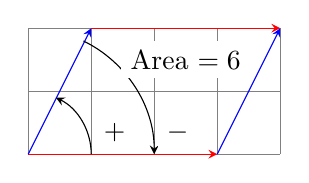
\begin{tikzpicture}[scale=.8]
\draw[help lines,step=1cm] (0,0) grid (4,2);
\draw[->,>=stealth,red] (0,0) -- (3,0);
\draw[->,>=stealth,red] [shift={(1,2)}](0,0) -- (3,0);
\draw[->,>=stealth,blue] (0,0) -- (1,2);
\draw[->,>=stealth,blue] [shift={(3,0)}](0,0) -- (1,2);
\draw[->,>=stealth] (0:1cm)  node[above right=1pt,fill=white]{\normalsize $+$} arc (0:64:1cm) ;
\draw[<-,>=stealth] (0:2cm)  node[above right=1pt,fill=white]{\normalsize $-$} arc (0:64:2cm) ;
\node[fill=white] at (2.5, 1.5) {Area $=6$}; 
\end{tikzpicture}

\vspace{2pt}
$\begin{vmatrix}{\red 3}&{\blue 1}\\{\red 0}&{\blue 2}\end{vmatrix}=6$ and $\begin{vmatrix}\blue{1}&\red{3}\\\blue{2}&\red0\end{vmatrix}=-6$

   The determinant gives area and direction.
    }}
These two vectors give the edges of a parallelogram whose area is the determinant ($6$).  If we swap the order of the two vectors in the matrix, then the determinant of $\begin{bmatrix}1&3\\2&0\end{bmatrix}$ is $-6$.  The absolute value of the determinant is still the area, but the sign of the determinant depends on the order of the vectors. Starting at the first vector, if you can turn counterclockwise through an angle smaller than 180$^\circ$ to obtain the second vector, then the determinant is positive.  If you have to turn clockwise instead, then the determinant is negative.  This is often termed the ``right-hand rule'' since rotating the fingers of your right hand from the first vector to the second vector will cause your thumb to point up precisely when the determinant is positive.

\marginpar{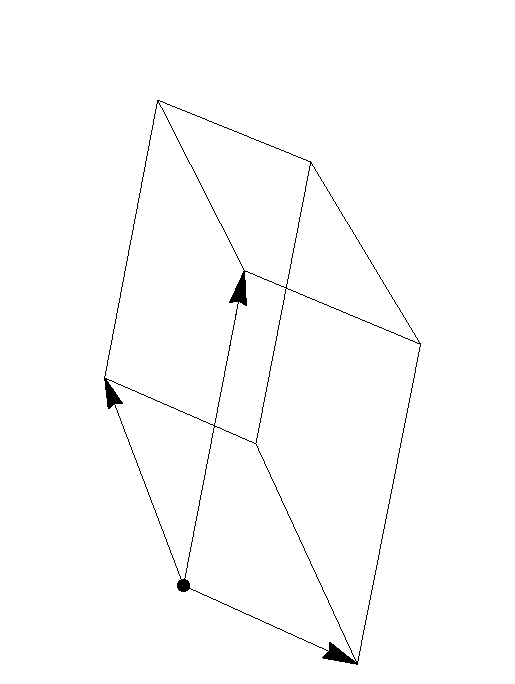
\includegraphics[width=\marginparwidth]{Arithmetic/support/det}

The determinant of a 3 by 3 matrix gives the volume of the parallelepiped created by using the columns of the matrix as the three parallel edges.} 
For a 3 by 3 matrix, the columns give the edges of a three-dimensional parallelepiped and the determinant produces the volume of this object. The sign of the determinant is related to orientation. If, using your right hand, you can place your index finger on the first vector, middle finger on the second vector, and thumb on the third vector, then the determinant is positive.  If you can't, then the determinant is negative.
\begin{example}
Consider the matrix $A = \begin{bmatrix}\cl{1\\0\\0}&\cl{0\\2\\0}&\cl{0\\0\\3}\end{bmatrix}$.  Starting from the origin, each column represents an edge of the rectangular box 
$0\leq x\leq 1$, 
$0\leq y\leq 2$, 
$0\leq z\leq 3$ with volume (and determinant) $V=lwh=(1)(2)(3)=6$. The sign of the determinant is positive because if you place your index finger pointing in the direction $(1,0,0)$ and your middle finger in the direction $(0,2,0)$, then your thumb points upwards in the direction $(0,0,3)$. 
If you interchange two of the columns, for example 
$B = \begin{bmatrix}\cl{0\\2\\0}&\cl{1\\0\\0}&\cl{0\\0\\3}\end{bmatrix}$, then the volume doesn't change since the shape is still the same. However, the sign of the determinant is negative because if you point your index finger in the direction $(0,2,0)$ and your middle finger in the direction $(1,0,0)$, then your thumb points down in the direction $(0,0,-3)$. If you repeat this with your left hand instead of right hand, then your thumb points up.
\end{example}

\subsection{Zero Determinants and Linear Dependence}
Because the determinant helps us find area in 2D, we can use this idea to help us understand when two vectors in 2D are linearly dependent.  
If two vectors are dependent, then one is a linear combination of the other, hence a multiple of the other.  
This means that the parallelogram formed by the two vectors has no area (as the two vectors lie on the same line).  
So if the vectors are dependent, the determinant is zero.  
Similarly, if the determinant is zero, then the vectors must lie on the same line and hence are linearly dependent.  
In 3D, three vectors being linearly dependent implies that one of the vectors lies in a plane or line spanned by the other two.
Any object in 3D that lies in a plane or line has no volume so the determinant is zero.  
Similarly, if the determinant of a 3 by 3 matrix is zero, then the column vectors must lie in the same plane and hence are linearly dependent. 
We now have a geometric interpretation for the key fact:
\marginpar{For a square matrix $A$, the following are equivalent:
\begin{enumerate}
	\item The determinant is zero.
	\item The columns are linearly dependent.
	\item The rref of $A$ is not $I$.
\end{enumerate}
}
\begin{quote}The determinant of a matrix is zero if and only if the columns are linearly dependent.\end{quote}
The homeworks asks you to compute determinants of matrices as well as row reduce them so that you can verify this fact in various settings. 
Notice that the columns of a square matrix are linearly independent if and only if the reduced row echelon form of the matrix is the identity matrix. 
This shows us that the determinant of a square matrix is nonzero if and only if the reduced row echelon form of the matrix is the identity matrix. 




\section{The Matrix Inverse}
\marginpar{See Section \ref{identity matrix}, page \pageref{identity matrix}}Recall that the identity matrix $I$ behaves in matrix multiplication like the number 1 behaves in regular multiplication.  
When we solve the equation $ax=b$ with numbers, we multiply both sides by $a^{-1}$ to obtain $x=a^{-1}b=\frac{1}{a}b$. 
The multiplicative inverse of $a$ is simply $1/a$, because $a\frac1a=\frac1a a=1$.
We have been studying linear systems of the form {$A\vec x=\vec b$}. 
\marginpar{If $A$ is a matrix, we \emph{never} write $\frac{1}{A}$ because matrix multiplication is not commutative.}% 
It would be nice if we could just divide both sides by {$A$}, but there is no such thing as division by a matrix in general.
If we look only at square matrices, then sometimes it is possible to find a matrix {$B$} such that {$BA=AB=I$}, the identity matrix. 
If such a matrix {$B$} exists, then multiplying both sides of {$A\vec x = \vec b$} on the left by the matrix {$B$} yields $BA\vec x = B\vec B$, or $I\vec x = \vec x = B\vec b$. The matrix {$B$} is then called the \define[matrix!inverse]{inverse} of {$A$}, and we write it as $A^{-1}$, the same symbol we used with regular multiplication. \marginpar{The solution to $A\vec x= \vec b$ is $\vec x=A^{-1}\vec b$, if $A^{-1}$ exists.}When an inverse exists, the solution to $A\vec x = \vec b$ is simply $\vec x = A^{-1}\vec b$.

To find an inverse, we will start by considering a general 3 by 3 matrix. Once we are done, we will know how to find the inverse of any $n$ by $n$ matrix or determine it does not exists.  
If an inverse exists, then write $A^{-1} = \begin{bmatrix}
c_{11}&c_{12}&c_{13}\\ 
c_{21}&c_{22}&c_{23}\\ 
c_{31}&c_{32}&c_{33} 
\end{bmatrix} $. Then the equation $AA^{-1}=I$ requires that the 3 matrix equations
$$A\begin{bmatrix} c_{11}\\ c_{21}\\c_{31}\end{bmatrix} = \begin{bmatrix} 1\\0\\0\end{bmatrix},\quad
A\begin{bmatrix} c_{12}\\ c_{22}\\c_{32}\end{bmatrix} = \begin{bmatrix} 0\\1\\0\end{bmatrix},\quad \text{ and }
A\begin{bmatrix} c_{13}\\ c_{23}\\c_{33}\end{bmatrix} = \begin{bmatrix} 0\\ 0\\1\end{bmatrix}$$
each have a solution, or that $(1,0,0), (0,1,0),$ and  $(0,0,1)$ are all linear combinations of the columns of $A$. This requires that we reduce all three augmented matrices
$$
\begin{bmatrix}[ccc|c]
a_{11}&a_{12}&a_{13}&1\\ 
a_{21}&a_{22}&a_{23}&0\\ 
a_{31}&a_{32}&a_{33}&0 
\end{bmatrix}
\quad\quad
\begin{bmatrix}[ccc|c]
a_{11}&a_{12}&a_{13}&0\\ 
a_{21}&a_{22}&a_{23}&1\\ 
a_{31}&a_{32}&a_{33}&0 
\end{bmatrix}
\quad\quad
\begin{bmatrix}[ccc|c]
a_{11}&a_{12}&a_{13}&0\\ 
a_{21}&a_{22}&a_{23}&0\\ 
a_{31}&a_{32}&a_{33}&1 
\end{bmatrix}.
$$
If the first three columns are all pivot columns, then the row operations required to reduce all three matrices will be identical, and none of the 4th columns will be pivot columns.  Rather than do three equivalent row reductions, we can solve all three simultaneously by creating the single augmented matrix 
$$\begin{bmatrix}[ccc|ccc]
a_{11}&a_{12}&a_{13}&1&0&0\\ 
a_{21}&a_{22}&a_{23}&0&1&0\\ 
a_{31}&a_{32}&a_{33}&0&0&1 
\end{bmatrix} $$\marginpar{If $A_{n\times n}$ is a square matrix, then the following are equivalent:
  \begin{enumerate}
  \item $A$ has an inverse $A^{-1}$.
  \item The columns of $A$ are linearly independent.
  \item The rank of $A$ is $n$
  \item The rref of $A$ is $I$.
  \item $|A|\neq 0$.
  \end{enumerate}

The following are also equivalent:
\begin{enumerate}
\item $A$ does not have an inverse  
\item The columns of $A$ are linearly dependent.
\item The rank is less than $n$
\item The rref of $A$ is not $I$ (there is a row of zeros along the bottom).
\item $|A|=0$.
\end{enumerate}
}or in compact form $\begin{bmatrix}[c|c]A &I\end{bmatrix}$. We now reduce this larger matrix to reduced row echelon form and obtain $\begin{bmatrix}[c|c]I &B\end{bmatrix}$, which tells us the coordinates of $(1,0,0)$, $(0,1,0),$ and  $(0,0,1)$ relative to the columns of $A$. 
The columns of the augmented portion $B$ on the right are the solutions to the three original systems, hence are the columns of $A^{-1}$.

To summarize, an inverse exists precisely if the augmented system $[A\mid I]$ reduces to $[I\mid A^{-1}]$. 
\begin{itemize}
\item If the identity matrix appears in the left block in the rref, the inverse matrix appears is in the right block and the original columns of $A$ are a linearly independent set.
\item If the left block of the augmented matrix does not reduce to the identity matrix, then the matrix $A$ does not have an inverse and the original columns of $A$ are a linearly dependent set.
\end{itemize}
Later we will show that having an inverse is equivalent to having a nonzero determinant and having a rank which equals the number of columns.

\begin{example}\label{ex inverse}
To find the inverse of 
$\begin{bmatrix} 1&2\\3&4\end{bmatrix}$,
we reduce 
$\begin{bmatrix}[cc|cc] 1&2&1&0\\3&4&0&1\end{bmatrix}$.  
Reduction gives 
$\begin{bmatrix}[cc|cc] 1&0&-2&1\\0&1&3/2&-1/2
\end{bmatrix}$. 
The inverse is the right block  
$ \begin{bmatrix} -2&1\\3/2&-1/2
\end{bmatrix}$. 
\marginpar{Examples involving larger matrices are in the homework. Remember that you can solve systems by finding an inverse of the coefficient matrix.}%
You can always check your result by computing $AA^{-1}$ to see if it is $I$, for example
$\begin{bmatrix} 1&2\\ 3&4\end{bmatrix} \begin{bmatrix} -2&1\\3/2&-1/2\end{bmatrix} 
=  \begin{bmatrix} 1&0\\0&1
\end{bmatrix}$. 
Using this inverse, the solution to the system 
$\begin{cases}1x+2y=4\\3x+4y=0\end{cases}$ is $A^{-1}\vec b 
= \begin{bmatrix} -2&1\\3/2&-1/2\end{bmatrix}
\begin{bmatrix}4\\0\end{bmatrix} 
=  \begin{bmatrix}-8\\6\end{bmatrix}$, so $x=-8$ and $y=6$.
\end{example}

Notice that if $A$ has an inverse, then $A\vec x=\vec b$ always has exactly one solution, $\vec x=A^{-1}\vec b$.  If a square matrix $A$ does not have an inverse, then the system $A\vec x=\vec b$ may have no solutions or may have infinitely many solutions.

\section{Eigenvalues and Eigenvectors}
In this section, we also assume that we are dealing with square matrices.  We will start by looking at an example to motivate the language we are about to introduce.  Consider the matrix
$A=\begin{bmatrix} 2&1\\1&2\end{bmatrix} $.  When we multiply this matrix by the vector 
$\vec x = \begin{bmatrix} 1\\1\end{bmatrix} $, 
we obtain 
$\begin{bmatrix} 2&1\\1&2\end{bmatrix} \begin{bmatrix} 1\\1\end{bmatrix} = \begin{bmatrix} 3\\3\end{bmatrix}=3 \begin{bmatrix} 1\\1\end{bmatrix}=3\vec x$. Multiplication by the matrix $A$ was the same as multiplying by the number 3! Symbolically, we have $A\vec x = 3\vec x$. 
Not every vector $\vec x$ satisfies this property, for example, multiplying $A$ by 
$\vec x = \begin{bmatrix} 1\\0\end{bmatrix} $ 
gives  
$\begin{bmatrix} 2&1\\1&2\end{bmatrix} \begin{bmatrix} 1\\0\end{bmatrix} = \begin{bmatrix} 2\\1\end{bmatrix}$, which is not a multiple of $\vec x = \begin{bmatrix} 1\\0\end{bmatrix} $. Our main goal in this section is to answer the following two questions:
\begin{enumerate}
	\item For which nonzero vectors $\vec x$ is it possible to write $A\vec x = \lambda \vec x$ for some scalar $\lambda$? (We will call these vectors eigenvectors.)
	\item Which scalars $\lambda$ satisfy $A\vec x = \lambda \vec x$ for some vector $\vec x$? (We will call these scalars eigenvalues.)
\end{enumerate}

Let's start with some vocabulary.
Let $A$ be a square $n\times n$ matrix. 
An \definemargin{eigenvector} is a nonzero vector $\vec x$ such that $A\vec x =\lambda \vec x$ for some scalar {$\lambda$} (i.e., multiplying $\vec x$ by the matrix $A$ is the same as multiplying $\vec x$ by the scalar $\lambda$).  The scalar $\lambda$ is called the \definemargin{eigenvalue} associated with the eigenvector $\vec x$.
Zero vectors are not eigenvectors because $A\vec 0=\lambda \vec 0$ no matter what $\lambda$ is (can you see that a particular nonzero eigenvector is only associated with one eigenvalue?).
We can rewrite the equation $A\vec x = \lambda \vec x$ as $\vec 0 = A\vec x-\lambda \vec x = A\vec x-\lambda I \vec x$ and then factor out the $\vec x$ to obtain 
$$(A-\lambda I)\vec x=\vec 0.$$ 
To solve this equation for $\lambda$, we need to find a scalar $\lambda$ so that there are nonzero solutions to the homogeneous system of equations $(A-\lambda I)\vec x=\vec 0$, or equivalently, we need to pick a $\lambda$ so that the columns of $A-\lambda I$ are linearly dependent. 
Recall that if the matrix $A-\lambda I$ has an inverse, then $(A-\lambda I)\vec x=\vec 0$ has only one solution, $\vec x=(A-\lambda I)^{-1}\vec 0=\vec 0$.  So if $A-\lambda I$ has an inverse, $\vec x$ cannot be an eigenvector.  With the correct $\lambda$, we know that $A-\lambda I$ has no inverse, so $\det(A-\lambda I)=0$. 
This last equation is the key equation we will solve since it does not contain the vector $\vec x$ anymore. 
The expression {$\det(A-\lambda I)$} is called the \definemargin{characteristic polynomial} of {$A$}.
It is a polynomial of degree {$n$} with variable $\lambda$, and hence there are at most {$n$} eigenvalues (which correspond to the roots of the polynomial). 
In summary, to find the eigenvalues and eigenvectors:
\begin{enumerate}
	\item we solve $\det(A-\lambda I) = 0$ for $\lambda$ to obtain the eigenvalues, and then
	\item for each eigenvalue $\lambda$, we solve $(A-\lambda I)\vec x=\vec 0$ to obtain the eigenvectors associated with $\lambda$.
\end{enumerate}
As a way to check your work, the following two facts can help.
\begin{itemize}
	\item \marginpar{The trace is the sum and the determinant is the product of the eigenvalues.}%
The sum of the eigenvalues equals the trace of the matrix (the sum of the diagonal elements).
	\item The product of the eigenvalues equals the determinant.
\end{itemize}
These are quick checks on your work.  You could have the wrong eigenvalues, but still have the sum equal the trace and the product equal the determinant.  However, if the sum of your computed eigenvalues is not the trace, or the product is not the determinant, you know there is an error somewhere.

\begin{example} \label{ex eigen1}
To find the eigenvalues of {$\begin{bmatrix} 2&1\\1&2\end{bmatrix} $}, first subtract $\lambda$ from each diagonal entry to get {$A-\lambda I=\begin{bmatrix} 2-\lambda&1\\1&2-\lambda\end{bmatrix} $}, and then find the determinant {$(2-\lambda)(2-\lambda)-1 = \lambda^2-4\lambda+3=(\lambda-1)(\lambda-3)$}. The roots are 1 and 3, so the eigenvalues are {$\lambda=1,3$}. As a check, the trace of this matrix is $2+2=4$ and the sum of the eigenvalues is $1+3$. Also, the determinant is $4-1=3$ which equals the product of the eigenvalues.  

When {$\lambda=1$}, we compute {$A-\lambda I =\begin{bmatrix} 1&1\\1&1\end{bmatrix} $}. We solve the equation  {$(A-\lambda I )\vec x=0$} by reducing the augmented matrix $\begin{bmatrix}[cc|c] 1&1&0\\1&1&0\end{bmatrix} $ to its rref $\begin{bmatrix}[cc|c] 1&1&0\\0&0&0\end{bmatrix} $.\marginpar{Since we are solving a homogeneous system $A\vec x = \vec 0$, we could avoid writing the last column of zeros.} Since $x_2$ is a free variable, we solve $x_1+x_2=0$ for $x_1$ to obtain the equations $x_1=-x_2$, $x_2=x_2$, and then write our solution in vector form 
$\begin{bmatrix} x_1\\x_2\end{bmatrix}= x_2\begin{bmatrix} -1\\1\end{bmatrix}$
 for some {$x_2\neq 0$} . There are infinitely many eigenvectors corresponding to $\lambda=1$. A particular eigenvector is  $\begin{bmatrix} -1\\1\end{bmatrix} $ and all the rest are nonzero linear combinations of this one. 

When {$\lambda=3$}, we compute {$A-\lambda I =\begin{bmatrix} -1&1\\1&-1\end{bmatrix} $}. Reducing  
$\begin{bmatrix}[cc|c] -1&1&0\\1&-1&0\end{bmatrix}$ gives
$\begin{bmatrix}[cc|c] 1&-1&0\\0&0&0\end{bmatrix}$, which means the eigenvectors are of the form $x_2\begin{bmatrix} 1\\1\end{bmatrix} $ for some {$x_2\neq 0$}. A particular eigenvector corresponding to $\lambda=3$ is $\begin{bmatrix} 1\\1\end{bmatrix} $, and all others are nonzero linear combinations of this one.
\end{example}

Finding eigenvalues and eigenvectors requires that we compute determinants, find roots of polynomials, and then solve homogeneous systems of equations. You know you are doing the problem correctly if you get infinitely many solutions to the system $(A-\lambda I)\vec x=0$ for each $\lambda$ (i.e. there is at least one row of zeros along the bottom of the rref matrix).

Eigenvalues and eigenvectors show up in many different places in engineering, economics, computer science, physics, chemistry, mathematics, and many other fields. We will be exploring how eigenvectors appear throughout linear algebra 
%and differential equations 
as the semester progresses.  For now we'll just focus on being able to find them.

\begin{example}\label{eigenvalueexample3} \label{ex eigen2}
Let's find the eigenvalues and eigenvectors of the matrix 
$A=\begin{bmatrix}2&1&4\\ 1&2&4\\ 0&0&1\end{bmatrix}$. 
Subtracting $\lambda$ from the diagonals gives 
$A-\lambda I=\begin{bmatrix}2-\lambda&1&4\\ 1&2-\lambda&4\\ 0&0&1-\lambda\end{bmatrix}$. The determinant of this matrix is easiest to compute if you expand along the third row to get $0 - 0 + (1-\lambda) \begin{vmatrix} 2-\lambda&1\\1&2-\lambda\end{vmatrix}$. Computing the 2 by 2 determinant gives $(1-\lambda)(\thinspace(2-\lambda)(2-\lambda)-1) = (1-\lambda)(\lambda-1)(\lambda-3)$,  so the eigenvalues are $1,1,3$ (1 is a repeated root). As a quick sanity check, the sum of our computed eigenvalues is $1+1+3=5$ and the trace of $A$ is $2+2+1=5$ as well.

When $\lambda=1$, we compute $A-\lambda I =\begin{bmatrix}1&1&4\\ 1&1&4\\ 0&0&0\end{bmatrix} $. Reducing the system  $(A-\lambda I )\vec x=0$ yields $\begin{bmatrix}[ccc|c]1&1&4&0\\ 0&0&0&0\\ 0&0&0&0\end{bmatrix}$, which has two free variables. The solution is $\begin{bmatrix} x_1\\x_2\\ x_3\end{bmatrix} = x_2\begin{bmatrix} -1\\1\\0\end{bmatrix}+x_3\begin{bmatrix} -4\\0\\1\end{bmatrix} $. Hence the eigenvectors are nonzero linear combinations of $\begin{bmatrix} -1\\1\\0\end{bmatrix}$ and $\begin{bmatrix} -4\\0\\1\end{bmatrix}$. Notice that all the eigenvectors can be obtained as linear combinations of two linearly independent eigenvectors, in part because $\lambda =1$ is a double root of the characteristic polynomial. 

When $\lambda=3$, we compute $A-\lambda I =\begin{bmatrix}-1&1&4\\ 1&-1&4\\ 0&0&-2\end{bmatrix}$. Next, reducing $\begin{bmatrix}[ccc|c]-1&1&4&0\\ 1&-1&4&0\\ 0&0&-2&0\end{bmatrix}$ yields $\begin{bmatrix}[ccc|c]-1&1&0&0\\ 0&0&1&0\\ 0&0&0&0\end{bmatrix} $, which has only one free variable . The solution is $\begin{bmatrix} x_1\\x_2\\ x_3\end{bmatrix} = x_2\begin{bmatrix} 1\\1\\0\end{bmatrix}$. The eigenvectors are nonzero linear combinations of $\begin{bmatrix} 1\\1\\0\end{bmatrix}$. Because $\lambda=3$ is a single root of the characteristic polynomial, all the eigenvectors can be obtained as linear combinations of one eigenvector.
\end{example}

%%% Local Variables: 
%%% mode: latex
%%% TeX-master: "../linear-algebra"
%%% End: 
